\documentclass[times, utf8, diplomski]{diplomski}
\usepackage{booktabs}
\usepackage{listings}
\usepackage{nameref}
\usepackage{hyperref}
\usepackage{xcolor}
\usepackage{graphicx}
\usepackage{float}
\usepackage{subfig}

\graphicspath{ {./imgs/} }

\renewcommand{\lstlistingname}{Kod}
\renewcommand{\lstlistlistingname}{Lista Kodova}
\lstset{language=C, tabsize=2}

\definecolor{codegreen}{rgb}{0,0.6,0}
\definecolor{codegray}{rgb}{0.5,0.5,0.5}
\definecolor{codepurple}{rgb}{0.58,0,0.82}
\definecolor{backcolour}{rgb}{0.95,0.95,0.92}

\lstdefinestyle{mystyle}{
    backgroundcolor=\color{backcolour},
    commentstyle=\color{codegreen},
    keywordstyle=\color{magenta},
    numberstyle=\tiny\color{codegray},
    stringstyle=\color{codepurple},
    basicstyle=\ttfamily\footnotesize\small,
    breakatwhitespace=false,
    breaklines=true,
    captionpos=b,
    keepspaces=true,
    numbers=left,
    numbersep=5pt,
    showspaces=false,
    showstringspaces=false,
    showtabs=false,
    tabsize=2
}

\lstset{style=mystyle}

\begin{document}

\thesisnumber{3155}

\title{Programska podrška za pouzdano prikupljanje podataka s ugradbenih sustava}

\author{Branimir Ričko}

\maketitle

\zahvala{Zahvaljujem se Lani, Tomiću, Frišču i Korenu na tome što su mi ispravili sve gršeke u radu, Andriji, najdražem bratu, na tome što mi je platil obranu diplomskom, Elizi na Kukuruznom čovjeku i svima ostalima koji su me motivirali da napišem ovaj rad do kraja. <3}

\tableofcontents

\chapter{Uvod}
Ugradbena računala nude brojne mogućnosti poboljšanja svakodnevice pojedinaca.
Njihove fizičke dimenzije i niska potrošnja čine ih dobrim kandidatima za stvaranje uređaja i strojeva koji su pametniji od onih proizvedenih u prošlom desetljeću.
Iako je bolja budućnost veoma blizu svima nama i iako postoje ugradbena računala koja nam omogućuju izradnju pametnijih stvari, proces izradnje nije nimalo trivijalan.
Ovaj se rad bavi navedenim procesom i analizom pouzdanosti istog.
Dokumentiran je postupak izrade jednostavnog sustava s ugradbenim računalom gdje je ugradbeno računalo STM32, koje čita podatke sa senzora i iste u realnom vremenu šalje na server.
U sklopu ovog rada izrađen je sustav koji sadrži ugradbeno računalo koje je povezano Bluetoothom na računalo i šalje očitanja s raznih senzora koji su povezani s mikrokontrolerom.
Opisane su značajke STM32L4 mikrokontrolera isto kao i glavni dijelovi Bluetooth standarda.
Objašnjena je komunikacija između mikrokontrolera i Bluetooth modula.
Navedeni su protokoli koji se koriste u komunikaciji između mikrokontrolera i senzora koji su povezani s mikrokontrolerom.
Izgrađeno je programsko rješenje koje se izvršava na STM32L4 mikrokontroleru.
Izgrađeno je programsko rješenje koje se izvršava na računalu na kojem je pokrenut Linux operacijski sustav.
Uspješno je ostvarena komunikacija programskog rješenja na mikrokontroleru i programskog rješenja na računalu.
Pouzdano se šalju podaci s akcelerometra i žiroskopskog senzora s mikrokontrolera na računalo.

\chapter{Ugradbena računala}
Ugradbena računala su računala malih dimenzija i niske potrošnje. Dimenzije takvih računala su veličine nekoliko centimetara, a češće su još i manje.
Električna potrošnja često se mjeri u miliamperima i to u najgorim slučajevima kad je računalno opterećenje najveće.
U situacijama kada obavlja minimalan rad potrošnja često pada na svega nekoliko mikroampera.
Razlikuju se od običnih računala po tome što često odrađuju samo jedan zadatak koji nije previše kompleksan.
Zadatak u ovom radu koji obavlja ugradbeno računalo je čitanje podataka s raznih senzora i slanje istih na računalo korištenjem drugog ugradbenog
računala kojem je jedini zadatak slanje podataka korištenjem Bluetooth protokola na računalo.
Pravilna implementacija sustava s ugradbenim računalom omogućuje izradu baterijskih uređaja koji bez ikakve intervencije korisnika mogu raditi desetljećima \cite{holosys}. 
Glavni nedostatak je otežana izrada takvih sustava. Posebno važno kod izrade takvih sustava je smanjenje memorijske i vremenske složenosti.
Dodatno, potrebno je obratiti pažnju na vrijeme koje ugradbeno računalo provodi u aktivnom stanju i smanjiti ga koliko god je moguće.
Sve to zahtijeva od programera da bude pažljiv kod izrade svakog dijela sustava.


\section{STM32}
STM32 \cite{STM32L476JG} je ugradbeno računalo. U ovom radu STM32 koristi se kao primjer računala na kojem je moguće razvijati pouzdan sustav.
Specifično, korišten je STM32L476JG mikroupravljač.
Glavne karakteristike STM32L476JG mikroupravljača su Arm Cortex M4 32-bitna jezgra koja ima takt od 80MHz-a.
Također, ima ugrađen 1MB flash memorije i 128KB statičke RAM memorije.
Ima podršku za mnogo komunikacijskih protokola (u ovom radu od iznimne važnosti bio je SPI komunikacijski protokol.)
Najvažnije od svega je iznimno niska energetska potrošnja.

\section{Sensortile}
Sensortile \cite{sensortile} je integrirana pločica na kojoj se nalazi STM32L4 mikrokontroler i nekoliko senzora. U ovom radu koristi se Sensortile pločica kao fizičko okruženje za razvoj pouzdanog ugradbenog sustava.
 
\begin{figure}[H]
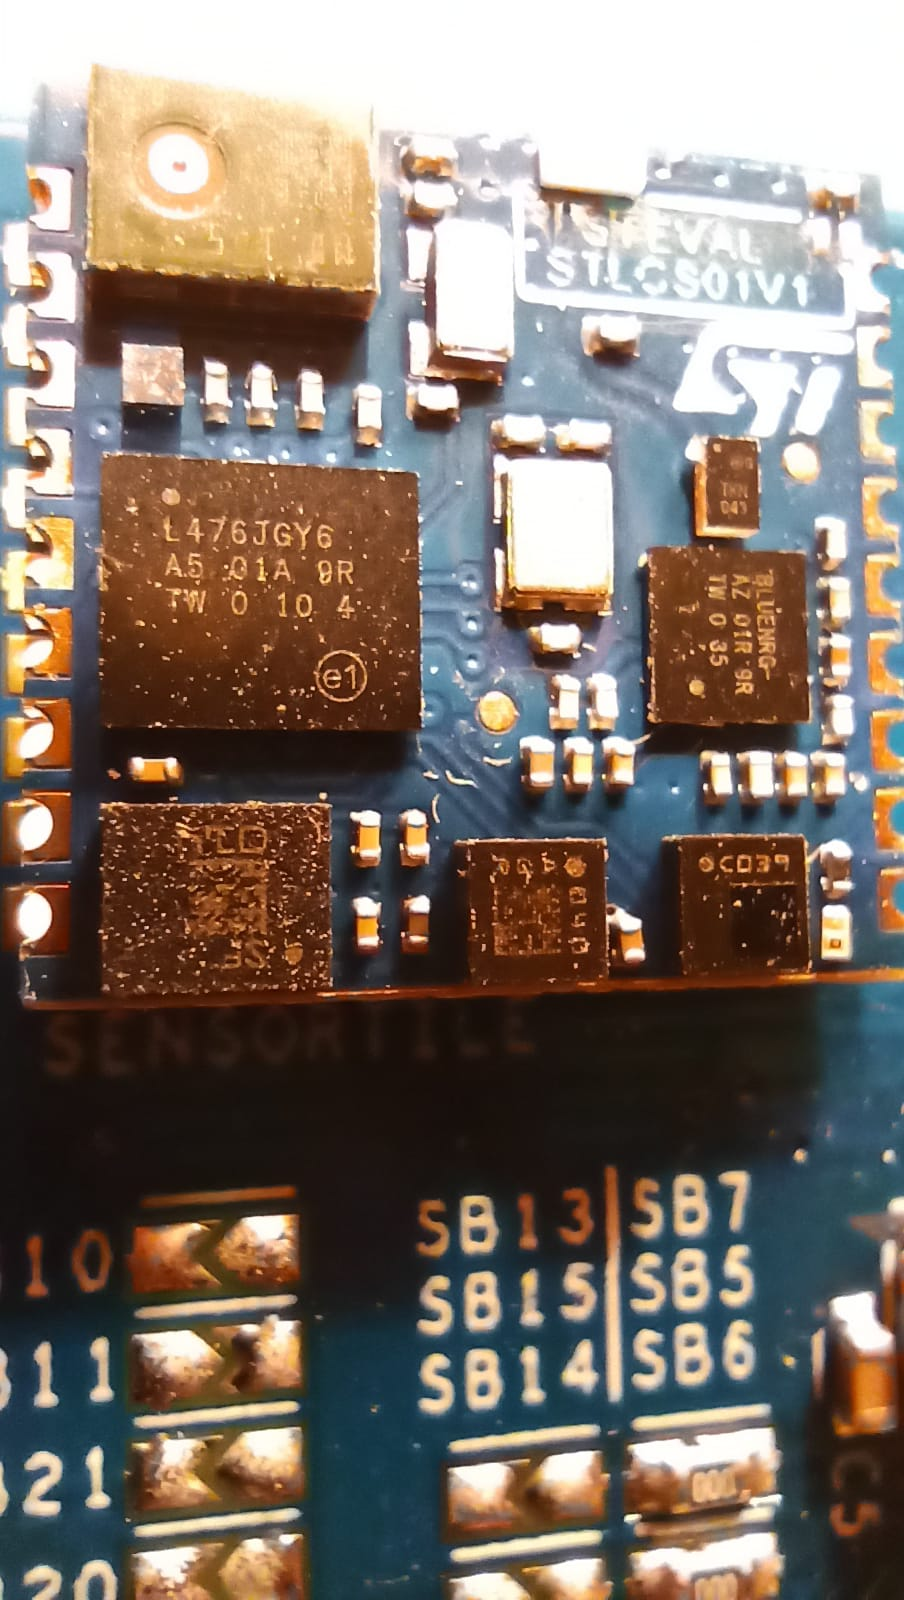
\includegraphics[scale=0.14]{tile_close.jpeg}
\centering
\caption{Sensortile ploćica}
\end{figure}

\subsection{LSM6DSM}
LSM6DSM \cite{LSM6DSM} je integrirani system-in-package koji sadrži 3-osni digitalni akcelerometar i žiroskop. Skala akcelerometra može biti podešena na ±2/±4/±8/±16g. Kutna brzina može biti podešena na
±125/±245/±500/±1000/±2000 stupnjeva po sekundi.

\subsection{LSM303AGR}
LSM303AGR je integrirani system-in-package koji sadrži 3-osni digitalni akcelerometar i 3-osni magnetometar. Skala akcelerometra je podesiva na
±2/±4/±8/±16g. Magnetometarski senzor ima dinamički raspon do ±50 gausa. Koristi I\(^2\)C ili SPI sučelje za komunikaciju.

\subsection{LPS22HB}
LPS22HB je integrirani system-in-package koji sadrži digitalni barometar. Koristi I\(^2\)C ili SPI sučelje za komunikaciju.

\subsection{MP34DT05-A}
MP34DT05-A je integrirani system-in-package koji sadrži digitalni mikrofon. Koristi I\(^2\)C sučelje.

\subsection{BlueNRG-MS}
BlueNRG-MS \cite{BlueNrgMs} je integrirani system-in-package koji sadrži Cortex M0 ARM jezgru i mogućnost Bluetooth 4.1 komunikacije.
Cijeli paket troši maksimalno 1mA za 1dBm izlazne snage. Za komunikaciju s glavnim mikrokontrolerom kositi se SPI komunikacija.

\subsubsection{Povezivanje BlueNRG-a sa STM32L4 microkontrolerom}
BlueNRG je Bluetooth module koji se nalazi na Sensortile pločici. Komunicira s STM32L4 mikrokontrolerom pomoću SPI protokola.
Svi razmijenjeni podaci između STM32L4 mikrokontrolera i BlurNRG modula koriste format prijenosa koji sadrži zaglavlje i tijelo poruke.
Zaglavlje poruke označava koliko je okteta BlueNRG spreman primiti te koliko je okteta željan poslati. Tijelo poruke sadrži informacije definirane Bluetooth standardnom.
Postoji pet signala koji povezuju Bluetooth module i STM32 mikrokontroler:

\begin{itemize}
  \item Odabir čipa (engl. \textit{Chip select CS}) - mikrokontroler stavlja na logičku nulu da označi da BlueNRG smije komunicirati.
  \item Takt (engl. \textit{Clock}) - mikrokontroler odrađuje takt kojim će komunicirati
  \item STM32 govori, BlueNRG sluša (engl. \textit{Master out, slave in})
  \item BlueNRG govori, STM32 sluša (engl. \textit{Master in, slave out})
  \item Podaci su spremni (engl. \textit{Data ready}) - BlueNRG označava da su dostupni podaci koje STM32 može pročitati.
\end{itemize}

\subsection{Povezivanje s računalom}
Kako bi ugradbeno računalo obavljalo koristan posao potrebno ga je prvo pripremiti za programiranje.
U ovom radu ugradbeno računalo koje se programira je STM32L4, nalazi se na Sensortile pločici (slika \ref{fig:plocab}.2, dalje Pločica A) koja je povezana s malo većom pločicom (slika \ref{fig:plocab}.1, dalje Pločica B.)
Pločica A i B povezane su s nestandardnim konektorom koji pinove sa STM32L4 direktno prenosi na Pločicu B.
Konektor se može vidjeti na slici \ref{fig:plocab}.5.
Pločica B na sebi sadrži ST Link \cite{stlink} priključak koji služi za programiranje (slika \ref{fig:plocab}.4.)
Pločica B na sebi sadrži micro USB port koji služi isključivo za napajanje (slika \ref{fig:plocab}.3.)

\begin{figure}[H]
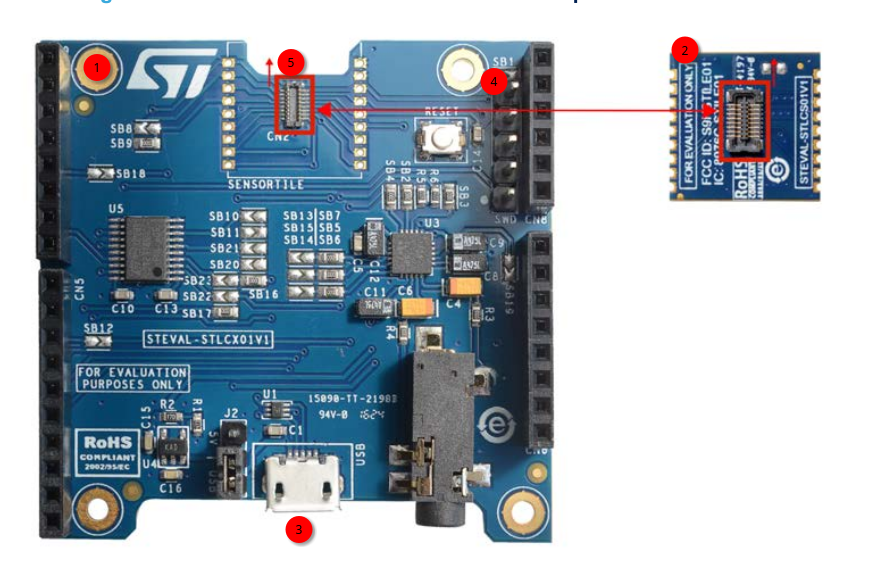
\includegraphics[scale=0.5]{PlocicaAiB.png}
\centering
\caption{Prikaz Pločice A i B jedna pored druge \cite{gettingstartedsensor}}
\label{fig:plocab}
\end{figure}

Pločica A i B nisu dovoljne za programiranje STM32L4 mikrokontrolera. Potrebna je dodatna pločica koja je u ulozi programatora (slika \ref{fig:prog}.) U ovom radu korišteno je fizičko razvojno okruženje NUCLEO-F439ZI koje je služilo za programiranje STM32L4 mikrokontrolera.
(dalje Pločica C.)

\begin{figure}[H]
  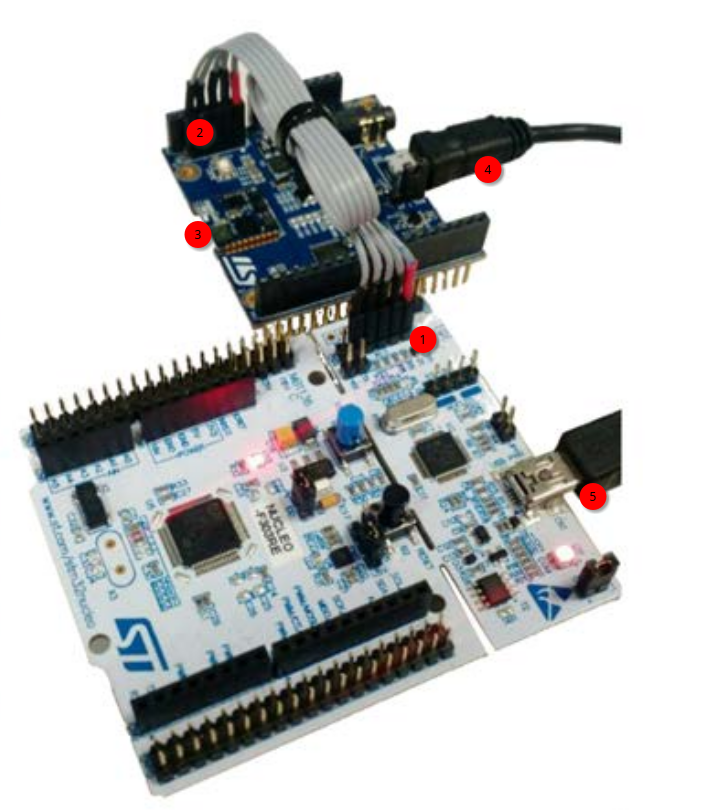
\includegraphics[scale=0.5]{connection_img.png}
  \centering
  \caption{Povezivanje STM32L4 mikrokontrolera s računalom \cite{gettingstartedsensor}}
  \label{fig:prog}
  \begin{enumerate}
    \item ST Link priključak na Pločici C.
    \item ST Link priključak na Pločici B.
    \item Nestandardni priključak koji povezuje Pločicu A i B.
    \item Usb priključak za napajanje Pločice B.
    \item Usb priključak za napajanje Pločice C i programiranje STM32L4 mikrokontrolera preko 1, 2, 3.
  \end{enumerate}
\end{figure}

\newpage

\section{Upravljanje događajima (engl. \textit{interrupts})}
Cortex M procesori posjeduju specifičan način upravljanjem događaja. Događaji su veoma bitni prilikom stvaranja ugradbenih sustava zato što omogućuju energetski efikasan dizajn sustava.
Umjesto aktivnog prozivanja od strane procesora \textit{nalazi li se što na nekoj sabirnici}, procesor može biti na hardverskoj razini obaviješten da je neka sabirnica promijenila stanje.
Kad se dogodi neki događaj izvodi se sljedeća procedura:

\begin{itemize}
  \item dovrši trenutnu instrukciju.
  \item spremi trenutno stanje procesora na stog.
  \item postavi LR registar na vrijednost \textbf{0xFFFFFFF9} (označava da procesor obrađuje događaj.)
  \item postavi IPSR registar na vrijednost broja događaja.
  \item postavi PC registar na lokaciju procedure koja obrađuje specifičan događaj.
\end{itemize}

\subsubsection{xPSR registar}

\begin{table}[H]
  \begin{center}
    \begin{tabular}{c|c|c|c|c||c||c||c|}
      \cline{2-8} & 31 & 30 & 29 & 28 & 24 & 9 & 5-0\\
      \hline
      \multicolumn{1}{|c|}{APSR} & N & Z & C & V & \multicolumn{3}{c|}{ } \\
      \hline
      \multicolumn{1}{|c|}{IPSR} & \multicolumn{6}{c||}{ } & Broj iznimke \\
      \hline
      \multicolumn{1}{|c|}{EPSR} & \multicolumn{4}{c||}{ } & T & a & \\
      \hline
    \end{tabular}
    \caption{Sadržaj xPSR registra}
  \end{center}
\end{table}

\newpage

\chapter{Bluetooth}

Bluetooth \cite{core41} je otvoren protokol koji definira bežični prijenos podataka na fizičkom sloju, na sloju veze i na mrežnom sloju.
Postoje komunikacijski standardi (npr. WiFi) koji zahtijevaju središnji uređaj na koji se povezuju svi ostali uređaji i kroz koji teče sva komunikacija između svakog para uređaja.
Bluetooth standard je osmišljen na načina da se dva uređaja povezuju i komuniciraju direktno jedan s drugim, bez korištenja središnjeg uređaja.

\section {Fizička razina}
Na fizičkoj razini Bluetooth protokol koristi Gausijansku binarnu digitalnu frekvencijsku modulaciju (engl. \textit{2GFSK modulation}) \cite{GBFSK}.
GBFSK je diskretna modulacija s dva stanja (1 bit/simbol.)
Za razliku od ostalih diskretnih modulacija s više diskretnih područja, binarna digitalna modulacija otpornija je na šumove i zahtjeva manju snagu za prijenos jednog simbola.
WiFi 7 standard podržavat će digitalnu modulaciju s 4096 diskretnih stanja \cite{wifimax} (12 bita/simbol.)
Cijena koju će novi WiFi standard platiti kompliciranijom modulacijom je smanjena otpornost na šum i kompliciranija izvedba uređaja.
Cijena koju Bluetooth protokol plaća s jednostavnijom modulacijom je manja teoretska propusnost.
Teoretska propusnost Bluetooth 4.2 LE protokola je 1Mbit/s \cite{maxtrough} dok će WiFi 7 protokol podržavati teoretsku propusnost od 46 Gbit/s.
Na podatkovnoj razini propusnost od 1Mbit/s s Bluetoothom 4.2 LE protokolom nije ostvariva zbog potreba sinkronizacije, enkripcije, konzistentnosti, pouzdanosti i proširivosti koje Bluetooth standard osigurava.
Uzevši u obzir sve nepodatkovne informacije potrebne za ispravan rad Bluetooth protokola, maksimalna teoretska propusnost je 508kbit/s.
U ovom radu s BlueNRG modulom maksimalna ostvarena propusnost je 25kbit/s.
Bluetooth modul BlueNRG implementira Bluetooth standard 4.1 koji ne podržava proširenje maksimalne jedinice prijenosa (engl. \textit{MTU}) na više od 20 okteta, dodatno interval povezvanja (engl. \textit{connection interval}) nije moguće smanjiti na vrijednost manju od 7.5 milisekunda i maksimalno je moguće poslati dvije prijenosne jedinice u jednom intervalu povezivanja.
Uzevši sve to u obzir, teoretska maksimalna propusnost BlueNRG modula je 42kbit/s.

\section{Bluetooth podsustavi}
Bluetooth standard definira podsustave koje moraju implementirati svi uređaji koji podržavaju Bluetooth. Neki važniji su definirani u ovom odlomku.

\subsection{GAP}
Bluetooth \textbf{G}eneric \textbf{A}ccess \textbf{P}rofile.
GAP definira uloge (engl. \textit{roles}) u Bluetooth standardu. Uloge koje postoje su oglašivač (engl. \textit{Advertizer}), skener (engl. \textit{Scanner}), sporedna (engl. \textit{Slave}) i glavna (engl. \textit{Master}) uloga. Oglašivačka i skener uloga vrše razmjenu informacija isključivo u smjeru od oglašivača do skenera. Isto tako, nije potrebno eksplicitno spajanje uređaja.
Više skenera može slušati jednog oglašivača.

\subsection{GATT}
Bluetooth \textbf{G}eneric \textbf{ATT}ribue Profile definira koji podaci postoje na pojedinim Bluetooth uređajima. Definira tako da svaki uređaj ima svoje servise koje su identificirani s jedinstvenim brojem (engl. \textit{UUID}). UUID može biti veličine 16 okteta ili 2 okteta. Neki brojevi su rezervirani u Bluetooth standardu \cite{core41}.
Dodatno, GATT definira da svaki servis sadrži svoje karakteristične tokove (engl. \textit{characteristic stream}) koji su isto tako identificirani jedinstvenim brojevima. Svaki karakteristični tok dodatno sadrži informaciju o tome je li taj tok namijenjen za pisanje ili čitanje, može li se oglašavati na tom toku, veličinu podatka jednog elementa tog toka. Primjer definicije jednostavnog servisa koji definira bateriju nekog uređaja prikazan je na slici \ref{fig:gattexample}

\begin{figure}[H]
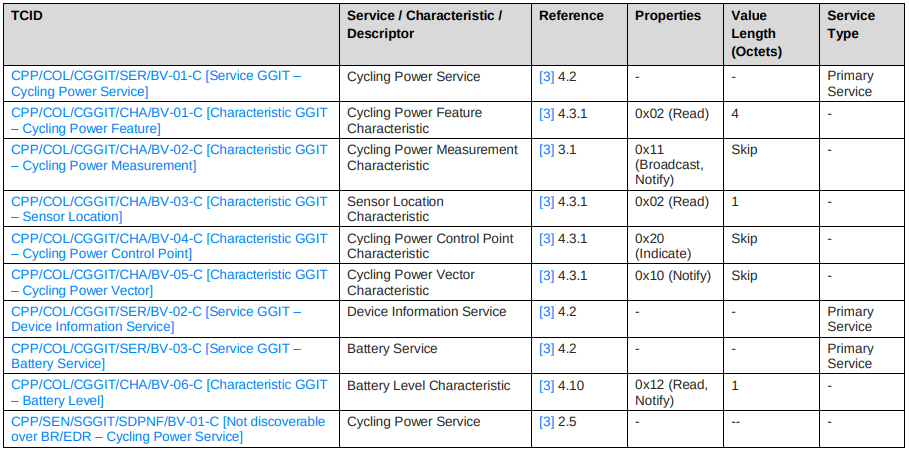
\includegraphics[width=\textwidth]{examplegatt_20230623_212042.png}
\centering
\caption{Tablica GATT servisa i karakterističnih tokova koji definiraju bateriju nekog uređaja}
\label{fig:gattexample}
\end{figure}

U ovom radu nije korišten niti jedan standardni servis, tj. korišten je servis kojeg je definirao autor rada. Standardni servisi tek postaju korisni ako korisnik želi izraditi uređaj koji će biti prepoznat od strane svih ostalih uređaja.

\subsection{L2CAP}
L2CAP je Bluetooth standard koji definira na koji način će dva Bluetooth uređaja razmjenjivati poruke na razini poveznice.

\subsection{HCI}
\textbf{H}ost \textbf{C}ontroller \textbf{I}nterface je Bluetooth standard koji definira u kojem se formatu razmjenjuju podaci od računala/mikrokontrolera do Bluetooth modula.

\subsection{ACI}
\textbf{A}pplication \textbf{C}ommand \textbf{I}nterface je standard kojeg definira tvrtka ST Microelectronics i koristi se kao sloj apstrakcije nad HCI slojem na STM32 mikrokontrolerima.


\section {Razmjena podataka između glavne i sporedne uloge}
Glavna i sporedna uloga zahtijevaju eksplicitno povezivanje (engl. \textit{pairing}.) Nakon povezivanja moguće je razmjenjivati poruke. Poruke je moguće razmijeniti na nekoliko načina:

\begin{itemize}
  \item Pisanje u karakteristični tok (engl. \textit{characteristic stream}) i čitanje iz istog.
  \item Oglašavanje promjena u karakterističnom toku.
  \item Oglašavanje promjena u karakterističnom toku uz potvrdu o primitku oglasa.
\end{itemize}

Pisanje i čitanje iz karakterističnih tokova zahtijeva dodatnu logiku za osiguranje prijenosa svih poruka. Ovaj način prijenosa radi na principu prozivanja.
Klijent koji čita podatak, bez dodatne intervencije, ne daje do znanja drugoj strani da je pročitao podatak,
ali uz dodatno programsko rješenje moguće je dati do znanja drugoj strani da je poruka pročitana.

\section {Oglašavanje promjena}
Razmjena poruka može se ostvariti oglašavanjem poruka. Oglašavanje poruka ostvaruje se tako da prilikom povezivanja uređaji sinkroniziraju satove i u točno određenim trenucima razmjene izmijenjene poruke. Dodatno, protokol bez intervencije korisnika koristi dvosmjernu komunikaciju za osiguravanje prijenosa poruke. Time se osigurava da će poruka biti isporučena. Dodatno, bez intervencije korisnika, na svaku poruku dodaje se CRC čime se osigurava točnost poruke.

\chapter{Programsko rješenje}
U sklopu ovog rada izrađeno je programsko rješenje koje se sastoji od djela koji se pokreće na STM32L4 mikrokontroleru i djela koji se pokreće na računalu s Linux operacijskim sustavom.
Programsko rješenje očitava podatke sa senzora koji su povezani sa STM32L4 mikrokontrolerom i te iste podatke prenosi na računalo korištenjem Bluetooth protokola.
U realnom vremenu računalo grafički iscrtava iste te podatke.

\section{Programsko rješenje za STM32L4 mikrokontroler}
Programsko rješenje za STM32L4 mikrokontroler pisano je u programskom jeziku C.
Na visokoj razini rješenje inicijalizira komunikacijske kanale prema senzorima i prema BlueNRG modulu.
Nakon toga pokreće se inicijalizacija postavki na BlueNRG modulu i BlueNRG se povezuje s računalom.
Nakon povezivanja počinju se očitavati vrijednosti senzora i isti podaci se prosljeđuju povezanom računalu.

U ovom radu postoje tri stanja u kojima se može nalaziti BlueNRG:

\begin{itemize}
  \item Neinicijalizirano
  \item Inicijalizirano
  \item Povezano
\end{itemize}

\subsection{Neinicijalizirano stanje BlueNRG-a}
Prilikom svakog ponovnog pokretanja, BlueNRG module se nalazi u \textbf{neinicijaliziranom} stanju. Sve interne vrijednosti postavljene su na inicijalne vrijednosti. Za ispravan rad BlueNRG modula potrebno je promijeniti neke vrijednosti. U ovom radu BlueNRG je u glavnoj ulozi. Postupak postavljanja BlueNRGa u glavnu ulogu u ovom radu izvršavaju se koraci opisani u kodovima od \ref{firstinit} do \ref{lastinit}.

\begin{lstlisting}[caption={Postavi MAC adresu}, label={firstinit}]
aci_hal_write_config_data(CONFIG_DATA_PUBADDR_OFFSET,
  CONFIG_DATA_PUBADDR_LEN, bdaddr);
\end{lstlisting}

\begin{lstlisting}[caption={Inicijaliziraj GATT podsustav}]
aci_gatt_init();
\end{lstlisting}

\begin{lstlisting}[caption={Inicijaliziraj GAP podsustav}]
aci_gap_init_IDB05A1(GAP_PERIPHERAL_ROLE_IDB05A1, privary_enabled, device_name_len, &service_handle, &dev_name_char_handle, &appearance_char_handle);
\end{lstlisting}

\begin{lstlisting}[caption={Postavi ime kojim će se predstavljati ostalim Bluetooth uređajima.}]
aci_gatt_update_char_value(state->service_handle,
  state->dev_name_char_handle,
  0, sizeof(name) - 1, (uint8_t *)name);
\end{lstlisting}

\begin{lstlisting}[caption={Postavi autentifikacijske zahtjeve}]
aci_gap_set_auth_requirement(
  MITM_PROTECTION_NOT_REQUIRED, // uint8_t mitm_mode,
  OOB_AUTH_DATA_ABSENT,         // uint8_t oob_enable,
  NULL,                         // uint8_t oob_data[16],
  7,                    // uint8_t min_encryption_key_size,
  16,                   // uint8_t max_encryption_key_size,
  USE_FIXED_PIN_FOR_PAIRING,    // uint8_t use_fixed_pin,
  123456,                       // uint32_t fixed_pin,
  BONDING,                      // uint8_t bonding_mode
);
\end{lstlisting}

\begin{lstlisting}[caption={Postavljanje servisa koji sadrži karakteristične tokove}]
aci_gatt_add_serv(UUID_TYPE_128,
  service_uuid, PRIMARY_SERVICE,
  number_of_char_streams, &service_id);
\end{lstlisting}

\begin{lstlisting}[caption={Postavljanje karakterističnih tokova}]
aci_gatt_add_char(serviceHandle,
  UUID_TYPE_16,
  char_uuid,
  20,               // Velicina poruke
  CHAR_PROP_NOTIFY, // Komunikacija obavijestima
  security_flags,
  GATT_NOTIFY_ATTRIBUTE_WRITE,
  16,               // encryKeySize
  false,            // Is length variable
  &charHandle
);
\end{lstlisting}

\begin{lstlisting}[caption={Postavi snagu odašiljača}]
aci_hal_set_tx_power_level(1, 7);
\end{lstlisting}

\begin{lstlisting}[caption={Postavi odgovor na poruku otkrivanja (engl. \textit{discover message})}]
// Ne odgovaraj
hci_le_set_scan_resp_data(0, NULL);
\end{lstlisting}

\begin{lstlisting}[caption={Postavi stanje BlueNRG-a u stanje u povezivo stanje}, label={lastinit}]
aci_gap_set_discoverable(
  ADV_DATA_TYPE,     // uint8_t AdvType,
  ADV_INTERV_MIN,    // uint16_t AdvIntervMin,
  ADV_INTERV_MAX,    // uint16_t AdvIntervMax,
  PUBLIC_ADDR,       // uint8_t OwnAddrType,
  NO_WHITE_LIST_USE, // uint8_t AdvFilterPolicy,
  9,                 // uint8_t LocalNameLen,
  "\nBlueNRG",       // const char *LocalName,
  0,                 // uint8_t ServiceUUIDLen,
  NULL,              // uint8_t* ServiceUUIDList,
  0,                 // uint16_t SlaveConnIntervMin,
  0,                 // uint16_t SlaveConnIntervMax
);
\end{lstlisting}
\ \

Nakon uspješnog izvršavanja navedenog postupka, BlueNRG prelazi u \textbf{inicijalizirano} stanje.

\subsection{Inicijalizirano stanje BlueNRG-a}
U \textbf{inicijaliziranom} stanju nema komunikacije između BlueNRG i STM32 mikrokontrolera sve dok se BlueNRG ne poveže s nekim Bluetooth poduređajem. Nakon što se BlueNRG poveže s Bluetooth poduređajem, BlueNRG generira događaj kojim obavještava STM32 mikrokontroler da se stanje može postaviti u \textbf{povezano}.

\subsection{Povezano stanje BlueNRG-a}
Nakon povezivanja, bez eksplicitnog zahtjeva, razmjene se poruke između BlueNRG-a i Bluetooth poduređaja koji je na njega povezan. Specifično, razmjenju se poruke o maksimalnoj veličini poruke (engl. \textit{MTU}), način enkripcije, definicija servisa i karakterističnih tokova. Nakon razmjene tih poruka, STM32 mikrokontroler može početi slati poruke s mjernim podacima. Procedura slanja u ovom radu je definirana na sljedeći način:

\begin{enumerate}
  \item Odredi koji će se karakteristični tok sljedeći slati
\begin{lstlisting}[caption = {Procedura za odabir karakterističnog toka koji će sljedeći biti poslan}]
int blue_send_next(blue_char_collection_t* coll, int len) {
  if (coll->waiting_for_confirm != -1) return -1;
  int i = coll->last_sent;
  int n = len;
  while(n > 0) {
    ++i;
    i %= len;
    if (coll->streams[i].send_ticks < uwTick && !is_empty(i)) {
      coll->waiting_for_confirm = i;
      coll->last_sent = i;
      ++coll->sent_packets;
      return blue_send_char_stream(&coll->char_streams[i], i);
    }
    --n;
  }
  return -1;
}
\end{lstlisting}
  \item Čekaj odgovor BlueNRG-a je li poruka uspješno poslana.
    \begin{enumerate}
      \item Ako je uspješno poslana, vrati se na korak 1.
      \item Ako nije uspješno poslana, pošalji istu poruku ponovno i vrati se na korak 2.
    \end{enumerate}
\end{enumerate}


\subsection{Performanse BlueNRG modula}

Mjerenje propusnosti BlueNRG modula mjereno je korištenjem programa Wireshark \cite{wireshark}. Nakon povezivanja, Wireshark prikuplja dolazne podatke 100 sekundi te su nakon toga izbrojene poruke. U tablici \ref{perftable} nalaze se mjerenja koja su izvršena. Na slici \ref{fig:wireshark} prikazano je jedno mjerenje.

\begin{table}[H]
  \begin{center}
    \begin{tabular}[c]{l|l|l|l}
      \hline
      \multicolumn{1}{c|}{\textbf{Broj tokova}} &
      \multicolumn{1}{c}{\textbf{Veličina poruke (bajt)}} &
      \multicolumn{1}{c}{\textbf{Poruka/sekunda}} &
      \multicolumn{1}{c}{\textbf{Bajt/sekunda}} \\
      \hline
      1 & 16 & 142 & 2272 \\
      1 & 20 & 144 & 2880 \\
      2 & 20 & 162 & 3240 \\
      \hline
    \end{tabular}
  \caption{Bluetooth performanse}
  \label{perftable}
  \end{center}
\end{table}

\begin{figure}[H]
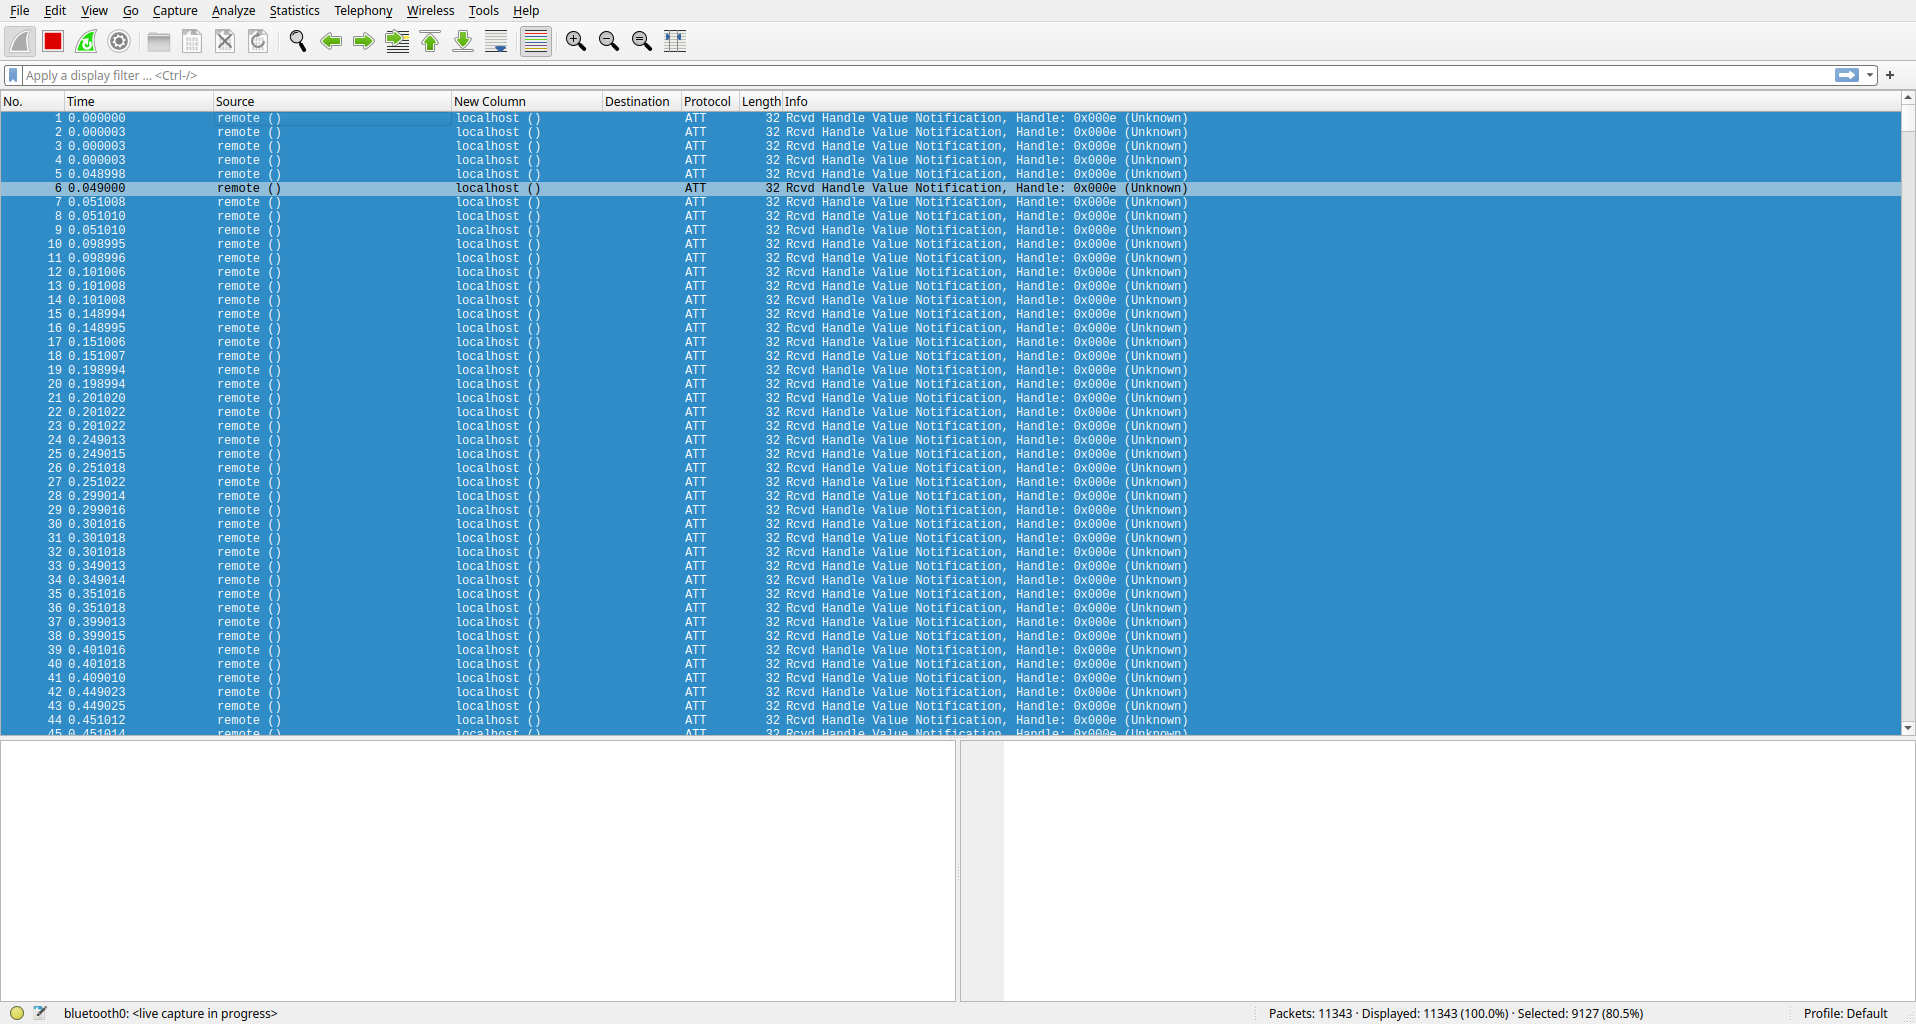
\includegraphics[width=\textwidth]{wireshark_100sec_20230622_225645.png}
\centering
\caption{Prikaza mjerenja korištenjem programa Wireshark \cite{wireshark}}
\label{fig:wireshark}
\end{figure}

U ovom radu testirano je nekoliko konfiguracija veličina paketa i broja tokova. Ukupna propusnost ne mijenja se značajno dodavanjem dodatnih tokova. Maksimalno kašnjenje nije mjereno, no pretpostavka je da nije veća od intervala spajanja (engl. \textit{connection interval}.) Interval spajanja definira Bluetooth poduređaj. U ovom radu bio je pet milisekundi.

\subsection{Ugradbeni program na Mikrokontroleru}
Ugradbeni program (engl. \textit{firmware}) za mikrokontroler pisan je u programskim jezicima C i C++. Pisan je na način da se sva komunikacija s Bluetooth BlueNRG modulom izvršava unutar događaja (engl. \textit{interrupt}). Nije korišten operativni sustav. Čitanje podataka sa senzora odvija se u glavnoj petlji programa. Postoji \textbf{struktura koja ima oblik reda} (engl. \textit{FIFO}) koja osigurava da se čitanje novih podatak sa senzora može odvijati neovisno o slanju istih Bluetoothom. Ista struktura opisana je kodom \ref{codefifo}.

\begin{lstlisting}[language=c++, caption={\textit{FIFO} struktura koja omogućuje neovisan dohvat novih podataka i slanje najstarijih}, label={codefifo}]
template<class T, size_t buffSize>
struct CircBuffer {
  T& push(T el) {
    auto& ret = buffer[pos++] = el;
    if (pos >= buffSize) pos = 0;
    if (len < buffSize) ++len;
    return ret;
  }
  T pop() {
    int index = (pos - len + buffSize) % buffSize;
    auto ret = buffer[index];
    if (len > 0) --len;
    return ret;
  }
  const T& peek() {
    int index = (pos - len + buffSize) % buffSize;
    return buffer[index];
  }
  size_t pos = 0;
  size_t len = 0;
  T buffer[buffSize] = {};
};
\end{lstlisting}

\subsubsection{Podatkovni protokol}
Sva podatkovna komunikacija se odvija od smjera mikrokontrolera do računalne aplikacije.
Koristi se više karakterističnih tokova (engl. \textit{characteristic stream}), svaki koristi način komunikacije s obavijestima, svaki obavještava s točno 20 podatkovnih okteta, svaki šalje točno dvije vrste poruka.
Jednom u tri sekunde kroz svaki tok šalje se kontrolna poruka, a ostatak vremena šalju se korisne poruke.
N-ti oktet kontrolne poruke sadrži vrijednost \textbf{(N \% 2) * 0xFF}, to jest prvi oktet ima vrijednost \textbf{0x00}, drugi \textbf{0xFF}, treći \textbf{0x00}, itd.
Svaki oktet kontrolne poruke ima tako definiranu vrijednost osim zadnja tri okteta.
Zadnja tri okteta kontrolne poruke opisuju strukturu korisnih poruka kao što je definiran tablicom \ref{datatable}.

\begin{table}[H]
  \begin{center}
    \begin{tabular}[c]{l|r}
      \multicolumn{1}{c|}{\textbf{Vrijednost opisnog okteta}} & 
      \multicolumn{1}{c}{\textbf{Definicija opisnog okteta}} \\
      \hline
      0b0000 & Podatak ne postoji \\
      0b0100 & jedan uint16 \\
      0b0110 & jedan int16 \\
      0b1000 & dva uint16 \\
      0b1010 & dva int16 \\
      0b1100 & jedan uint32 \\
      0b1110 & jedan int32 \\
      0b1111 & jedan float32 \\
      \hline
    \end{tabular}
  \caption{Značenje svakog kvarteta zadnjih šest kvarteta kontrolne poruke}
  \label{datatable}
  \end{center}
\end{table}

Jedna od poruka koja se šalje je poruka koja sadrži podatke prikupljene sa žiroskopskog senzor LSM6DSM. Struktura koja se puni opisana je u kodu \ref{codereadout}:

\begin{lstlisting}[language=c++, caption = {Definicija strukture koja se šalje Bluetoothom}, label={codereadout}]
 struct [[gnu::packed]]  GyroReadout {
  uint16_t temperature;
  int16_t acceleration[3];
  int16_t angular[3];
};
struct [[gnu::packed]]  GyroReadoutBLE {
  GyroReadout ro;
  uint16_t index;
  uint32_t timestamp;
};
\end{lstlisting}

Važno je napomenuti zašto je \textit{[[gnu::packed]]} atribut postavljen na svaku od struktura. Razlog stavljanja je raspored memorije.
Ako struktura nema taj atribut, svaka varijabla tipa \textit{GyroReadout} neće imati očekivanu veličinu, osim ako očekivana veličina nije upravo ona koja se dobije kad se dodaju dodatni okteti koji služe tome da podaci u memoriji uvijek budu spremljeni na način da ih je moguće pročitati s minimalnim brojem procesorskih ciklusa (engl. \textit{padding bytes}.)
U kontekstu serijalizacije, slanja i deserijalizacije ti okteti nisu važni i samo bi usporavali proces pouzdanog prijenosa podataka.
Navedena struktura puni se svakih 10 milisekundi pozivom metode navedene u kodu \ref{codegetreadout}.

\begin{lstlisting}[language=c++, caption={Dohvaćanje očitanja s LSM6DSM senzora}, label={codegetreadout}]
GyroReadoutBLE get_readout(void) {
  GyroReadout ro{};
  SPI_read(LSM6DSM_ACC_GYRO_OUT_TEMP_L,
    (uint8_t*)(&ro), sizeof(ro));
  return {ro, index++, uwTick}; // uwTick is global variable
                                // that is incremented in 
                                // some interrupt every 1ms.
}
\end{lstlisting}

Uzevši u obzir tipove vrijednosti od kojih se sastoji struktura \textit{GyroReadoutBLE} funkcija u kodu \ref{codecontroll} puni kontrolnu poruku za tok koji šalje \textit{GyroReadoutBLE} podatke.

\begin{lstlisting}[language=c++, caption={Funkcija koja puni kontrolnu poruku za žiroskopske podatke}, label={codecontroll}]
void fill_controll_message_gyro(uint8_t* buff) {
  for (int i = 0; i < 17; ++i) {
    buff[i] = (i % 2) * 0xFF;
  }
  buff[17] = 0x4A; //uint16, 2*int16
  buff[18] = 0xAA; //2*int16, 2*int16
  buff[19] = 0x4C; //uint16, int32
}
\end{lstlisting}

\section{Bluetooth na Linux operativnom sustavu}
Za testiranje pouzdanosti i kvalitete prijenosa preko Bluetootha potrebno je softversko rješenje koje pokreće na računalu. U ovom radu korišteno je rješenje koje se izvršava na Linux operativnom sustavu. Navedeni su neki softverski paketi koji olakšavaju rad s Bluetooth uređajima u Linux okolini.

\begin{table}[H]
  \begin{center}
    \begin{tabular}[c]{l|r}
      \multicolumn{1}{c|}{\textbf{Paket}} & 
      \multicolumn{1}{c}{\textbf{Opis paketa}} \\
      \hline
      dbus & Multipleksiranje komunikacije s jednim Bluetooth uređajem \\
      bluez-utils & Pomoćni programi za ispitivanje Bluetooth protokola \\
      bluez-libs & Biblioteke implementacijom raznih Bluetooth protokola \\
      bluez & Servis za automatsko upravljanje Bluetooth adapterima \\
      \hline
    \end{tabular}
  \caption{Lista paketa potrebnih za ispravan rad Bluetootha na Linux os-u}
  \end{center}
\end{table}

\subsection{Aplikacija za računalo}
Sama aplikacija na strani računala podijeljena je na dva djela. Dio aplikacije za popvezivanje Bluetoothom pisan je u programskom jeziku Python. Jezgra prvog djela je preuzeta od poznate Python biblioteke \textit{ble-serial} \cite{ble-serial}. Svrha prvog djela je spajanje Bluetoothom na uređaj i slušanje oglasa o promjeni stanja koje mijenja uređaj. Dodatno, dio aplikacije za povezivanje Bluetoothom prosljeđuje eksplicitno definirane podatke drugom djelu aplikacije preko UDP protokola \cite{firstPart}. Dio aplikacije za prikaz podataka prikuplja podatke od dijela aplikacije za povezivanje Bluetoothom i iste podatke grafički iscrtava \cite{secondPart}. Razlog razdvajanja aplikacije je to što programski jezik C pruža okruženje u kojem je moguće kreirati responzivno sučelje za grafički prikaz, a programski jezik Python omogućuje izrazito jednostavnu komunikaciju korištenjem Bluetooth protokola.

\subsubsection{Dio aplikacije za povezivanje Bluetoothom}
Dio aplikacije za povezivanje Bluetoothom napravljen je vrlo jednostavno. Kreira se UDP socket kao što je prikazano u kodu \ref{pyudpsock}. Pošalje se zahtjev preko dbus sustava da se Bluetoothom želi povezati s mikrokontrolerom kao što je prikazano u kodu \ref{pyconnect}. Nakon toga se pretplati na sve obavijesti sa svih servisa i karakterističnih tokova na mikrokontroleru kao što je prikazanu u kodu \ref{pysubscribe}. Prilikom svake obavijesti, izvršava se funkcija koja prosljeđuje dobivene podatke drugom dijelu aplikacije (kod \ref{relay}).

\begin{lstlisting}[language=python, caption={Kreiranje UDP socketa u Pythonu}, label={pyudpsock}]
client_socket = socket.socket(socket.AF_INET, socket.SOCK_DGRAM)
client_socket.settimeout(1.0)
addr = ("localhost", 42069)
\end{lstlisting}

\begin{lstlisting}[language=python, caption={Spajanje Bluetoothom na mikrokontroler}, label={pyconnect}]
ble = BLE_interface("hci0", None)
ble.set_receiver(receive_callback)
await ble.connect("02:80:E1:00:00:AA", "public", 16.0)
\end{lstlisting}

\begin{lstlisting}[language=python, caption={Pretplaćivanje na sve obavijesti sa svih servisa i karakterističnih tokova na mikrokontroleru}, label={pysubscribe}]
self.read_char = self.find_all_char(read_uuid)
r = [asyncio.Task(self.dev.start_notify(r, self.handle_notify)) for r in self.read_char]
await asyncio.wait(r)
\end{lstlisting}

\begin{lstlisting}[language=python, caption={Prosljeđivanje dobivene Bluetooth vrijednosti drugom dijelu aplikacije}, label={relay}]
p = DBParser()
def receive_callback(handle: BleakGATTCharacteristic, value: bytes):
    p.add_data(handle.handle, value)
    d = p.pop_data() # group_id, value 
    while d != None:
        client_socket.sendto(f"{d[1]};{d[0]}".encode(), addr)
        d = p.pop_data()
\end{lstlisting}

\subsubsection{Dio aplikacije za prikaz podataka}
Dio aplikacije za prikaz podataka nije povezan Bluetoothom. Rađen je jer je bilo potrebno validirati dobivene podatke. Grafički prikaz podataka taj zadatak drastično olakšava. Slika \ref{fig:graph} prikazuje stanje dijela aplikacije za prikaz podataka nakon nekoliko sekundi od početka prikupljanja podataka. 

\begin{figure}[H]
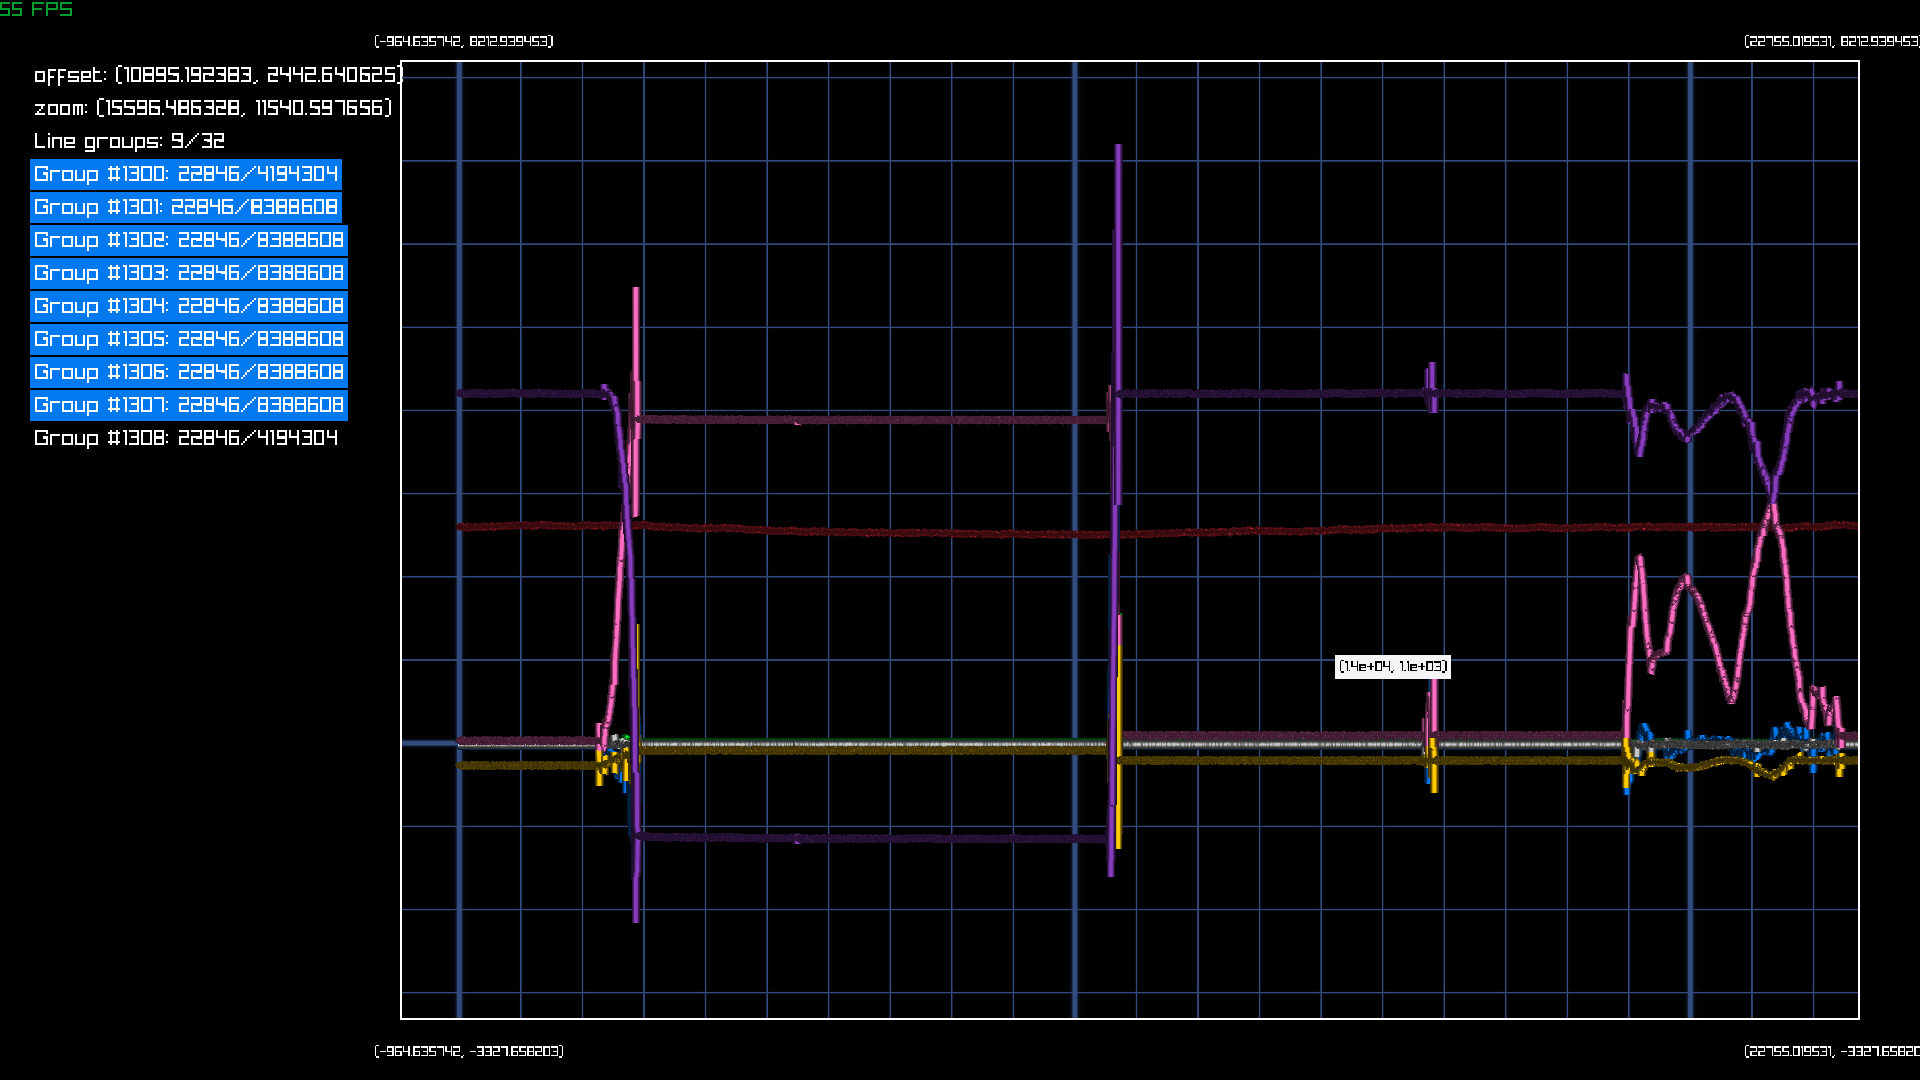
\includegraphics[width=\textwidth]{rlplot_allsensors_20230623_120537.png}
\centering
\caption{Prikaz dijela aplikacije za prikaz podataka koja iscrtava vrijednosti senzora u realnom vremenu}
\label{fig:graph}
\end{figure}

Rad cijelog sustava prikazan je u videu na adresi \url{https://youtu.be/AVqU0vSDVG8} \cite{videodemo}.

Izvorni kod programa za mikrokontroler, dio aplikacije za komunikacijom Bluetooth protokolom, aplikacija za prikaz podataka, dokumentacija i sve ostale skripte dostupne su u git repozitoriju na adresi \ \url{https://github.com/branc116/diplomski}.

\newpage
\chapter{Mjerenje pouzdanosti}
Dio ovog rada je mjerenje pouzdanosti sustava slanja očitanih podataka korištenjem Bluetootha. Mjerene metrike su:
\begin{enumerate}
  \item Broj izgubljenih paketa uzevši u obzir brzinu očitanja podataka
  \item Broj elemenata u strukturi koja ima oblik reda uzevši u obzir brzinu očitanja podataka
\end{enumerate}
U svim mjerenjima kapacitet strukture koja ima oblik reda je 128 elemenata.

\section{Broj izgubljenih paketa uzevši u obzir brzinu očitanja podataka}
U ovom radu mjeren je broj izgubljenih paketa uzevši u obzir brzinu očitanja podataka. Procedura kojom se mjerilo bila je:
\begin{enumerate}
  \item Postavnjanje željenog broja očitanja u izvorni kod ugradbenog programa
  \item Pokretanje ugradbenog sustava i aplikacije za prikupljanje podataka na računalu
  \item Čekanje sve dok aplikacija ne dobije 4000 očitanja
  \item Spremanje grafa izgubljenih pakata
\end{enumerate}

Na slici \ref{fig:packet_loss} prikazana su mjerenja izgubljenih pakata kad su se prikupljali podaci svakih 5 do 10ms.


\begin{figure}[H]
  \begin{tabular}{cc}
    \subfloat[10ms]{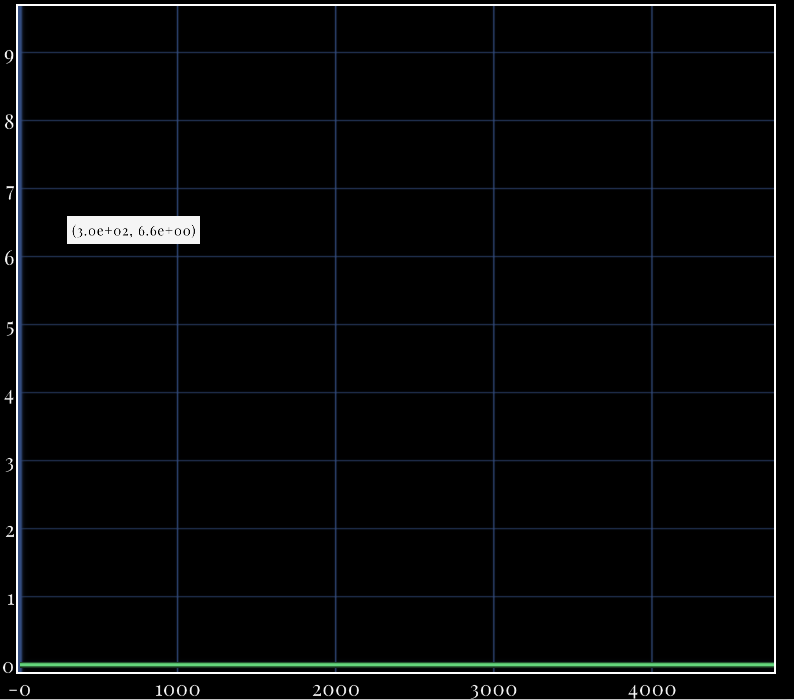
\includegraphics[width=2.8in]{packets_lost_every_10ms.png}} &
    \subfloat[9ms]{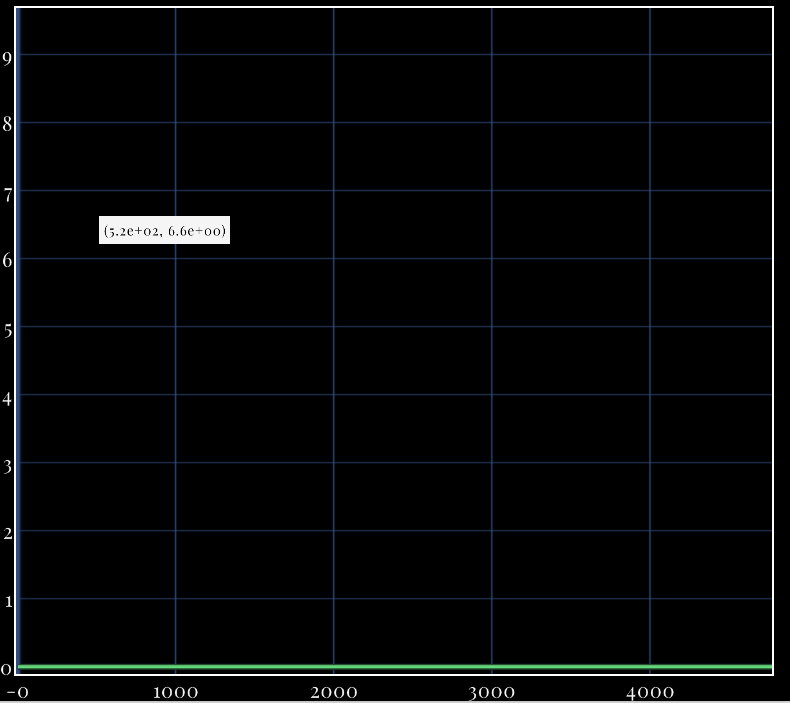
\includegraphics[width=2.8in]{packets_lost_every_9ms.png}} \\
    \subfloat[8ms]{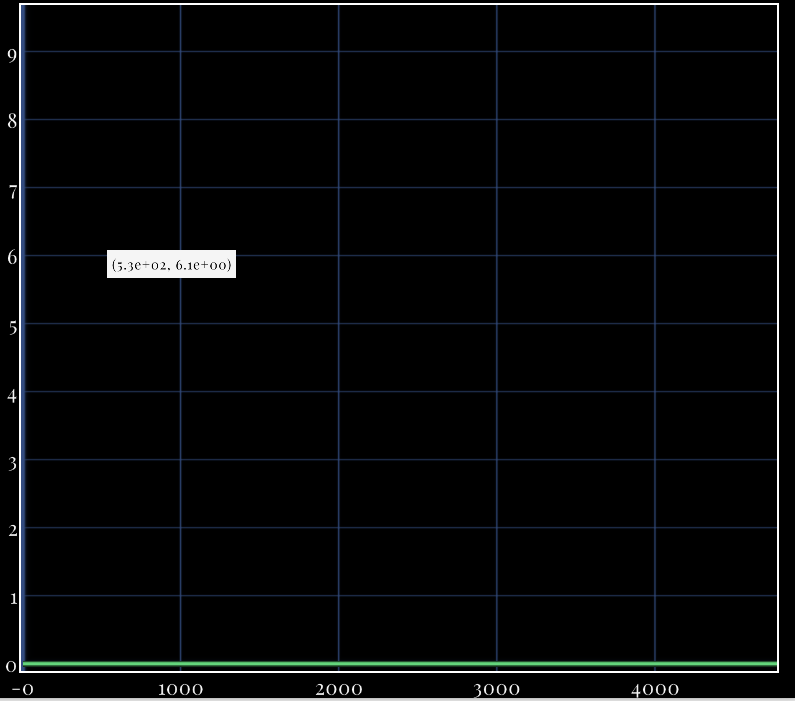
\includegraphics[width=2.8in]{packets_lost_every_8ms.png}} &
    \subfloat[7ms]{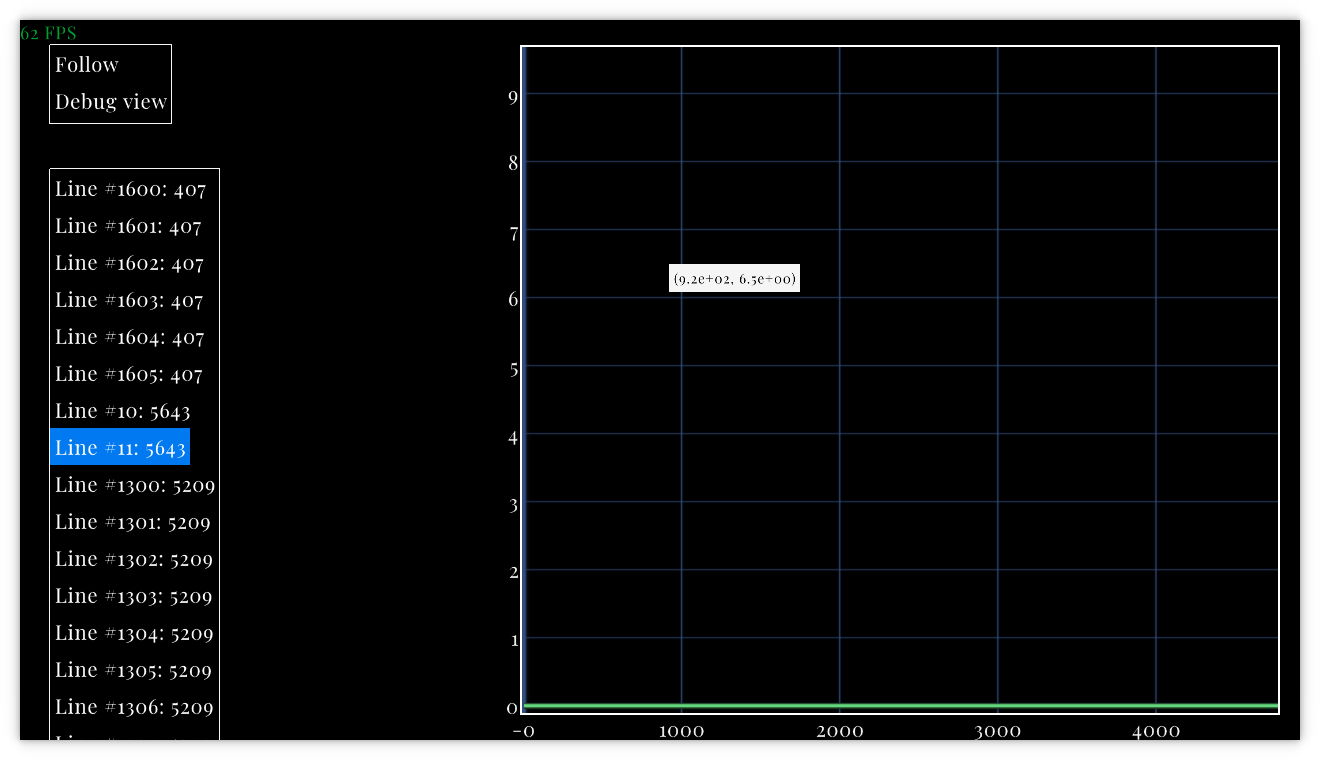
\includegraphics[width=2.8in]{packets_lost_every_7ms.png}} \\
    \subfloat[6ms]{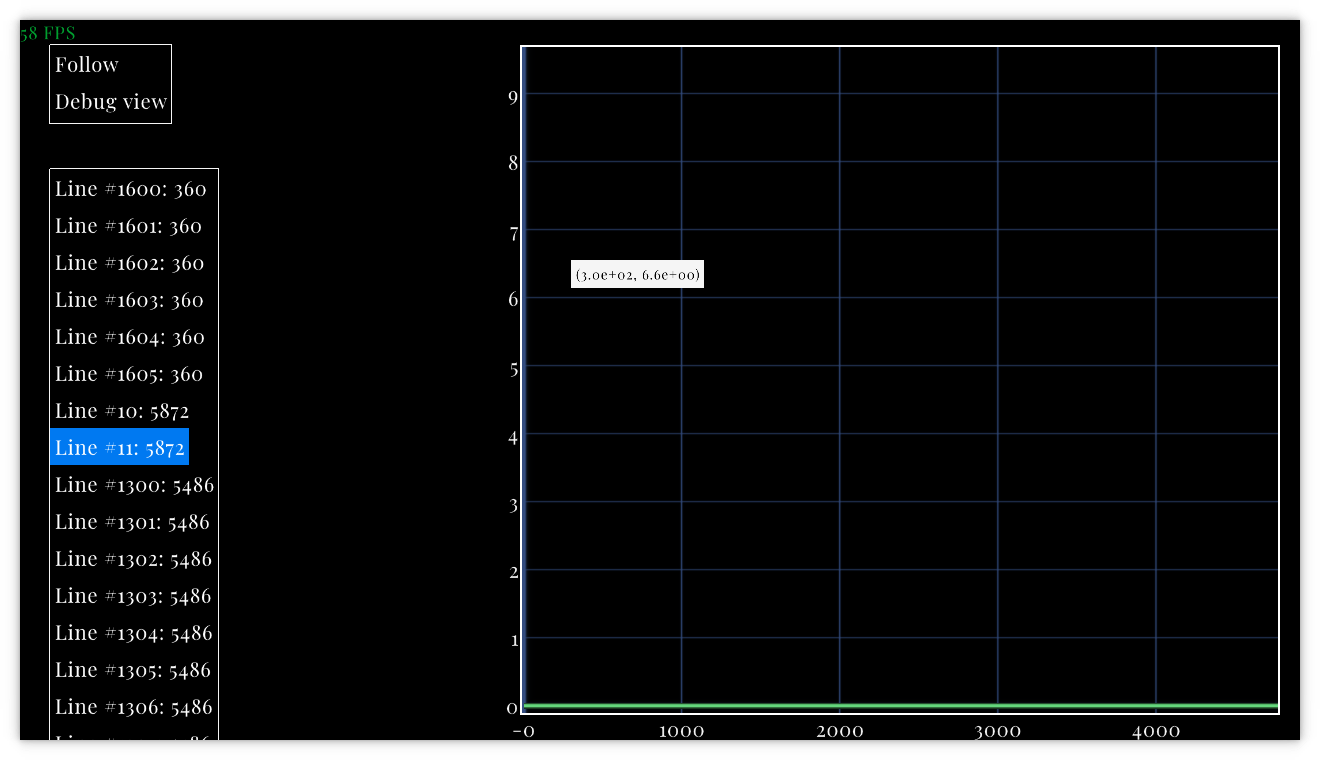
\includegraphics[width=2.8in]{packets_lost_every_6ms.png}} &
    \subfloat[5ms]{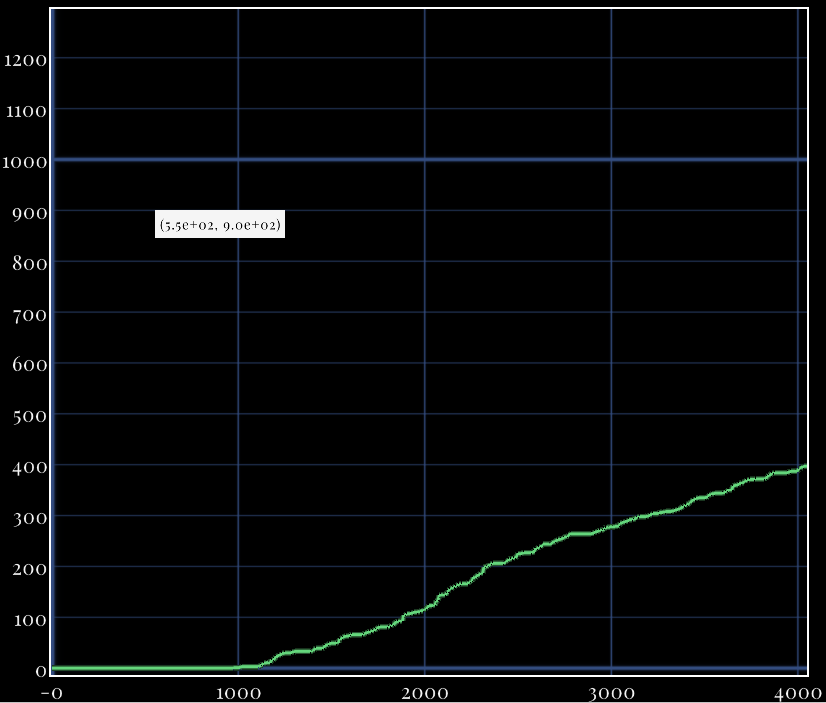
\includegraphics[width=2.8in]{packets_lost_every_5ms.png}}
  \end{tabular}
  \caption{Broj izgubljenih paketa uzevši u obzir brzinu očitanja podataka}
  \label{fig:packet_loss}
\end{figure}

Može se vidjeti da se paketi gube tek kada je interval očitanja podataka kraći od 6ms.
Dodatno, provedena su duža mjeranja kada je interval očitanja 5ms. Jedno gdje je broj očitanja bio 20`000 i dva gdje je broj očitanja bio 50`000.
Još jedno mjerenje provedeno je sa itervalom očitanja 6ms, ali u ovoj situaciji, autor rada je udaljavao i približavao ugradbeno računao od računala dok se provodilo mjerenje.
Slika \ref{fig:packet_loss_2} prikazuje ta mjerenja.
Na slici \ref{fig:packet_loss_2} se može primjetiti da broj izgubljenih paketa raste ukoliko se mikroupravljač udaljava od računala.

\begin{figure}[H]
  \begin{tabular}{cc}
    \subfloat[5ms]{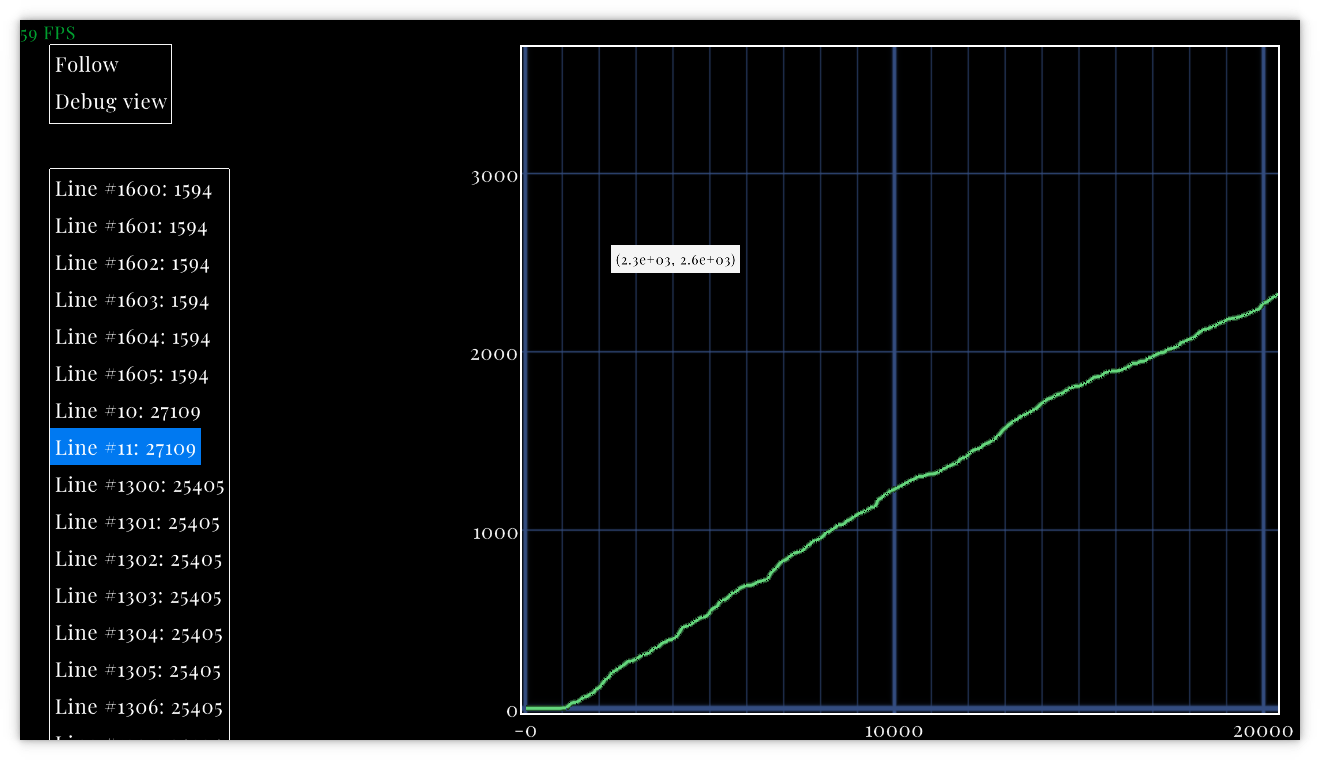
\includegraphics[width=2.8in]{packets_lost_every_5ms_20k.png}} &
    \subfloat[5ms]{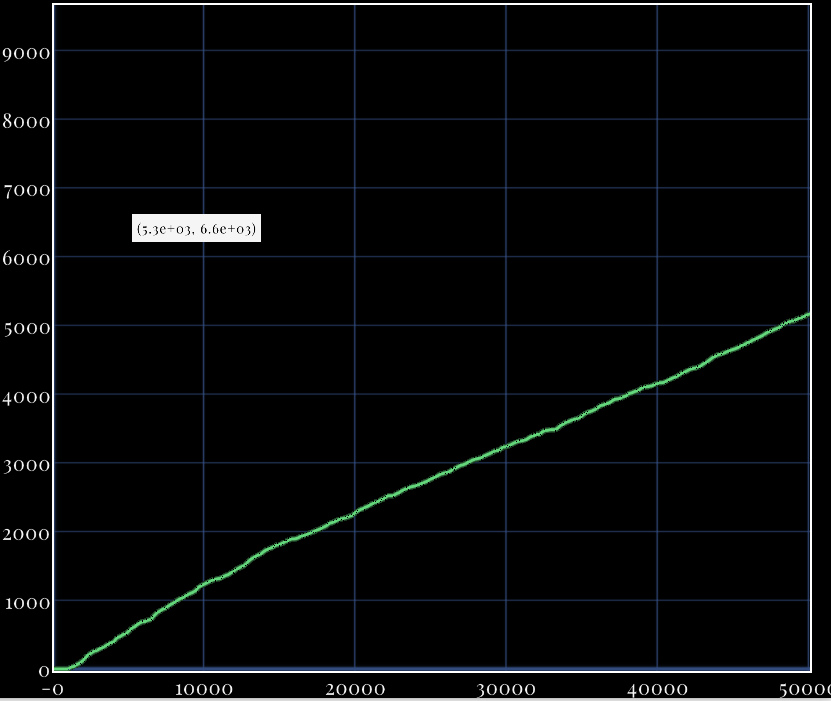
\includegraphics[width=2.8in]{packets_lost_every_5ms_50k.png}} \\
    \subfloat[5ms]{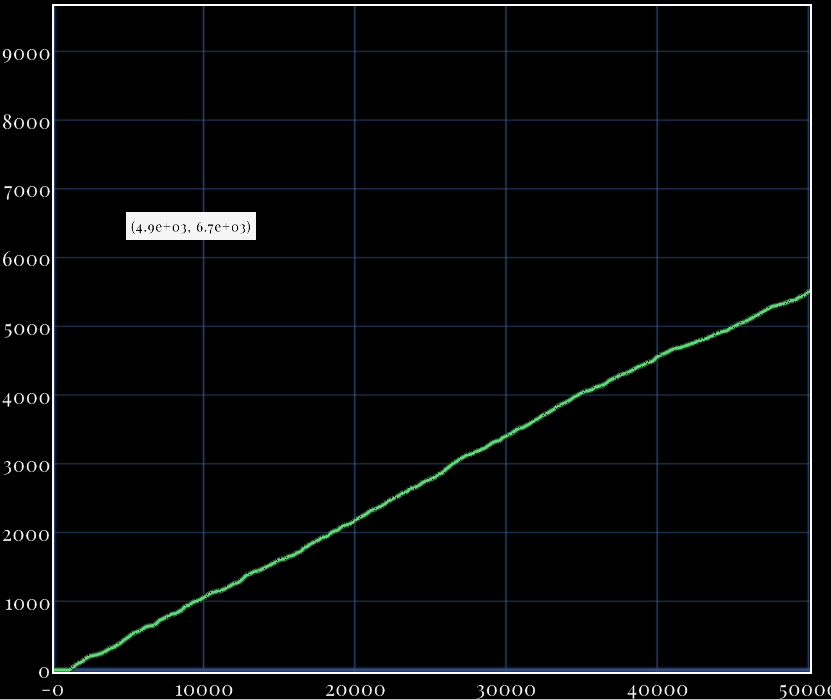
\includegraphics[width=2.8in]{packets_lost_every_5ms_50k_v2.png}} &
    \subfloat[6ms uz udaljavanje]{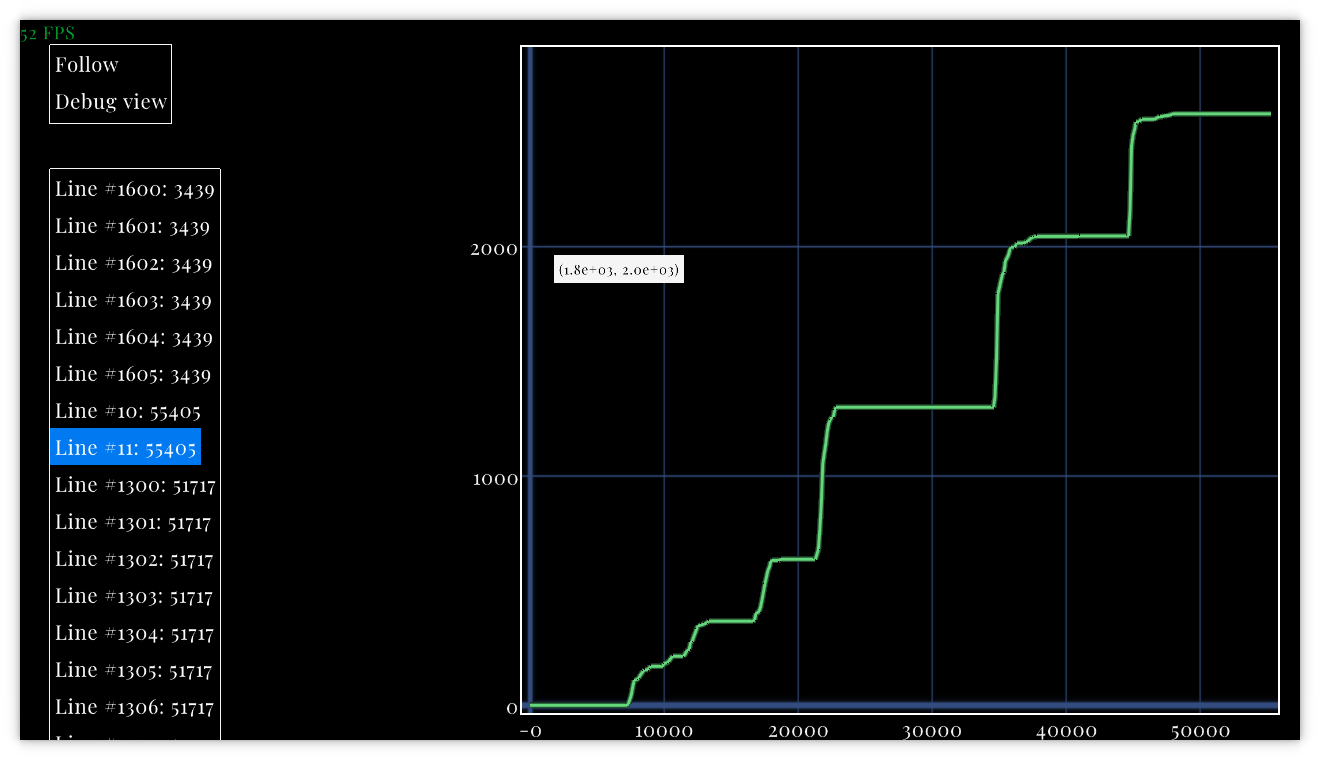
\includegraphics[width=2.8in]{packets_lost_every_6ms_with_walking.png}}
  \end{tabular}
  \caption{Broj izgubljenih paketa uz brzinu očitanja podataka od 5ms i 6ms}
  \label{fig:packet_loss_2}
\end{figure}

Provedena su još mjerenja s intervalom očitanja podataka od 4 milisekunde.
Na slikama \ref{fig:packet_loss_4_20} i \ref{fig:packet_loss_4_50} prikazani su rezultati tih mjerenja.

\begin{figure}[H]
  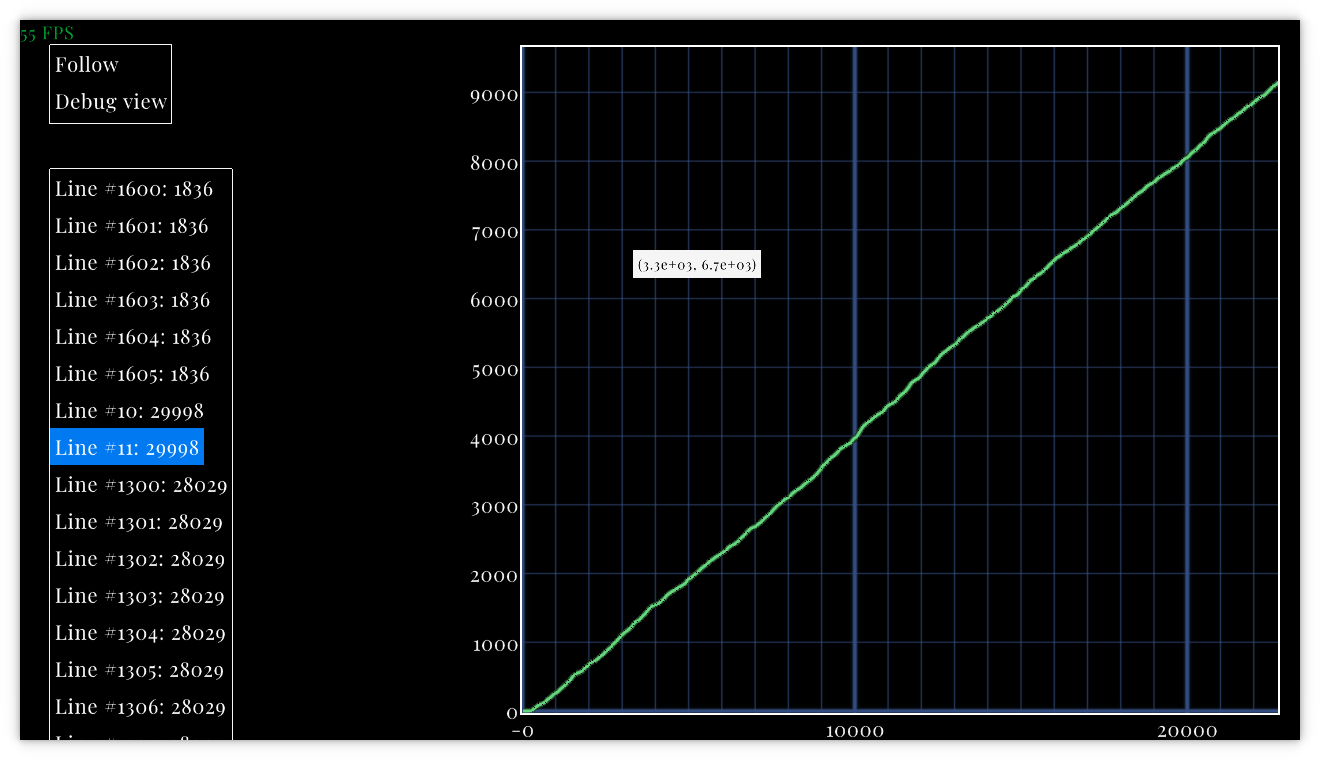
\includegraphics[width=\textwidth]{packets_lost_every_4ms_20k.png}
  \caption{Broj izgubljenih paketa uz brzinu očitanja podataka od 4ms. Dvadest tisuća očitanja.}
  \label{fig:packet_loss_4_20}
\end{figure}

\begin{figure}[H]
  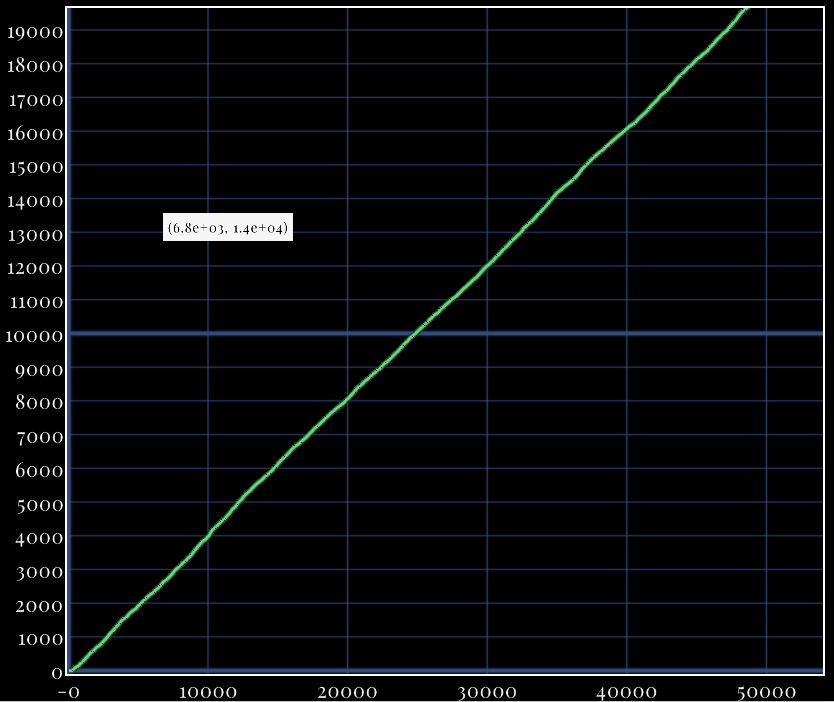
\includegraphics[width=\textwidth]{packets_lost_every_4ms_50k.png}
  \caption{Broj izgubljenih paketa uz brzinu očitanja podataka od 4ms. Pedeset tisuća očitanja.}
  \label{fig:packet_loss_4_50}
\end{figure}

Može se primjetiti da je broj izgubljenih paketa velik.

\section{Broj elemenata u strukturi koja ima oblik reda uzevši u obzir brzinu očitanja podataka}

Za provedbu ovog mjerenja implementiran je dodatni karakteristični tok koji šalje interne podatke o stanju mikroupravljača.
Specifično, jedan od podataka je broj elemenata u strukturi koja ima oblik reda.
Taj podatak je zanimljiv za promatrati je govori o tome koliko je Bluetooth mikroupravljač opterećen i može se vidjeti poveznica između broja izgbljenih paketa i broja elemenata u strukturi koja ima oblik reda.
Na slici \ref{fig:q_full} prikazani su rezultati mjerenja broja elementa uz intervale očitavanja od 5 do 10 milisekundi.

\begin{figure}[H]
  \begin{tabular}{cc}
    \subfloat[10ms]{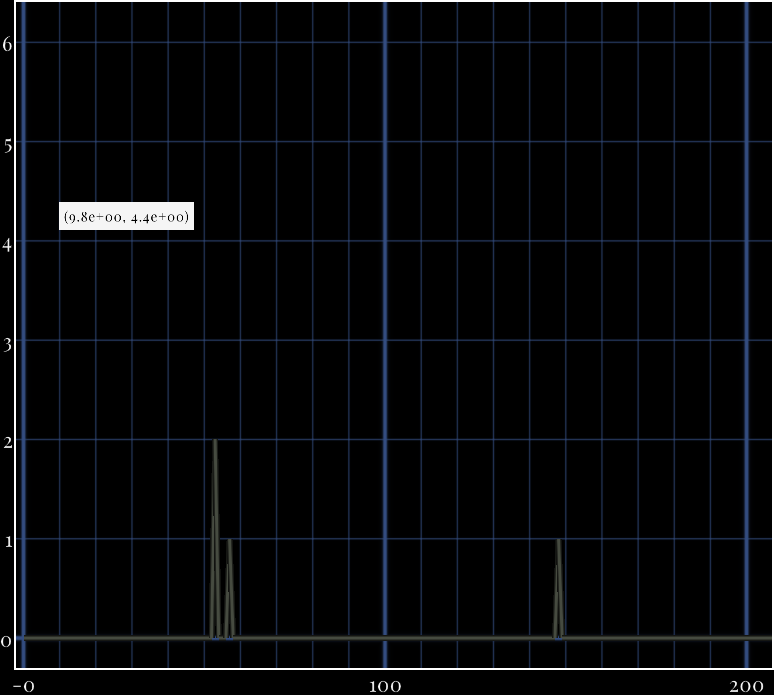
\includegraphics[width=2.8in]{q_full_ro_every_10ms.png}} &
    \subfloat[9ms]{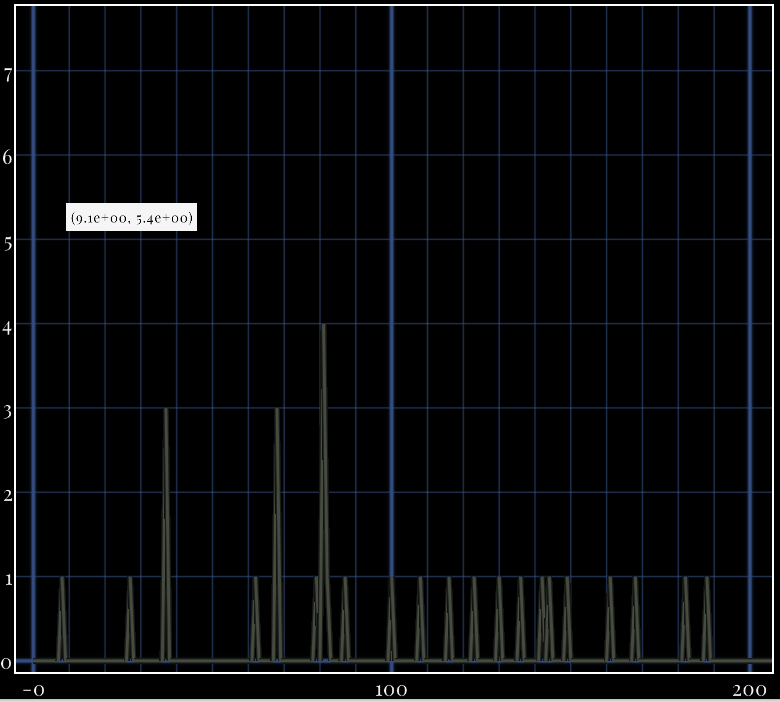
\includegraphics[width=2.8in]{q_full_ro_every_9ms.png}} \\
    \subfloat[8ms]{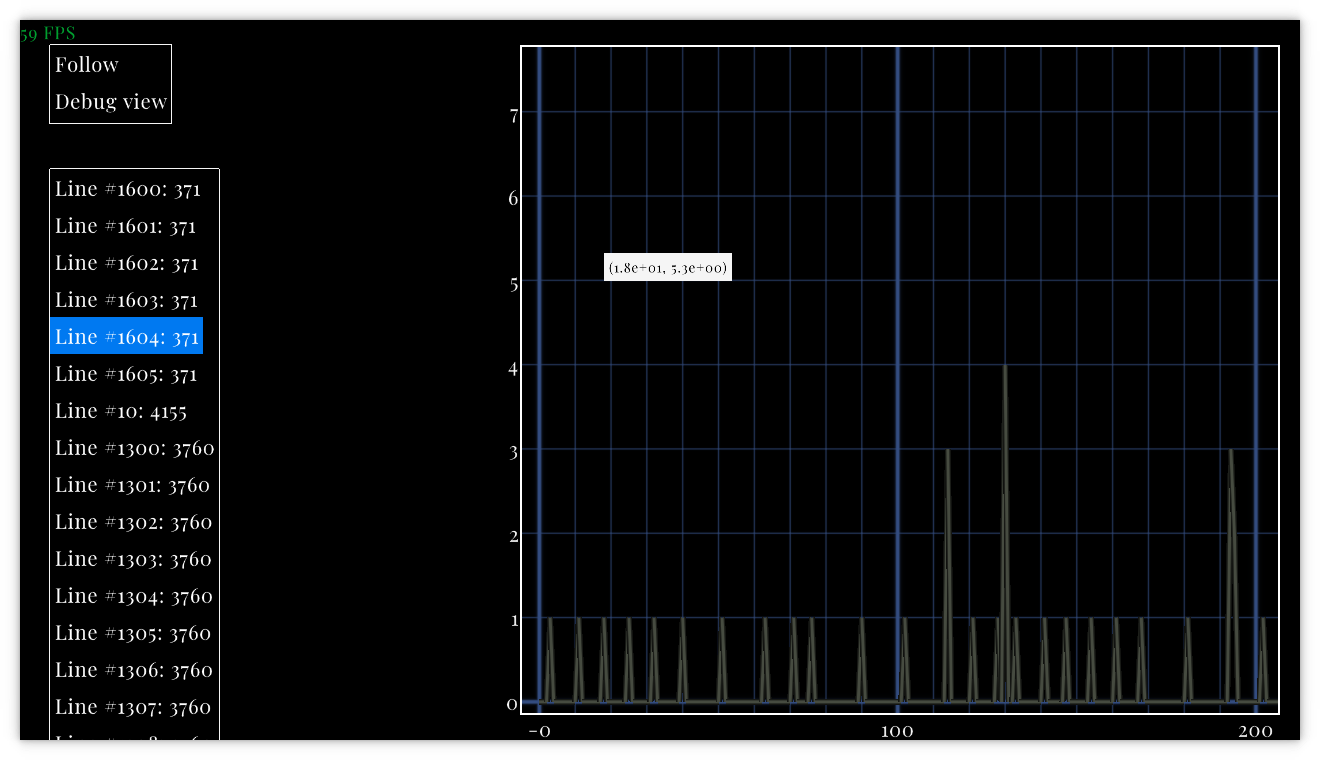
\includegraphics[width=2.8in]{q_full_ro_every_8ms.png}} &
    \subfloat[7ms]{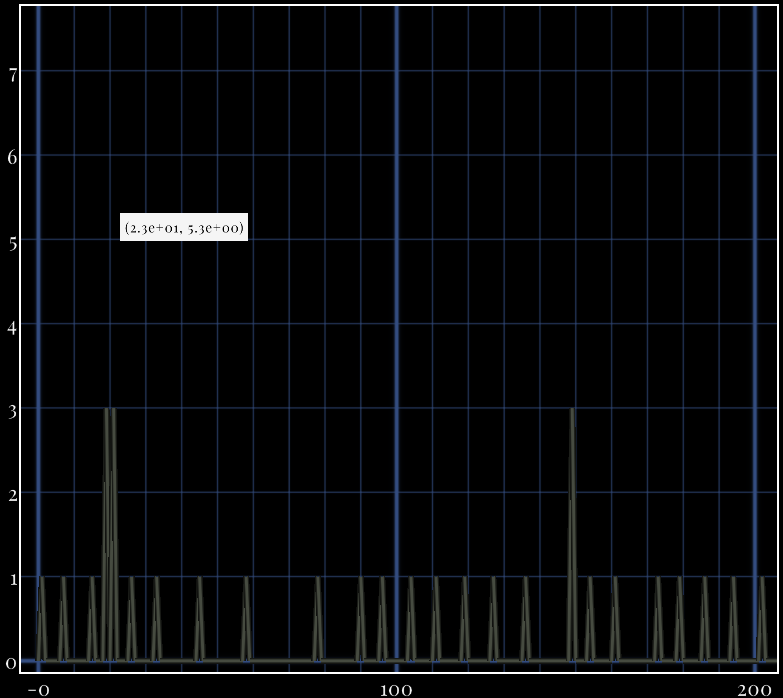
\includegraphics[width=2.8in]{q_full_ro_every_7ms.png}} \\
    \subfloat[6ms]{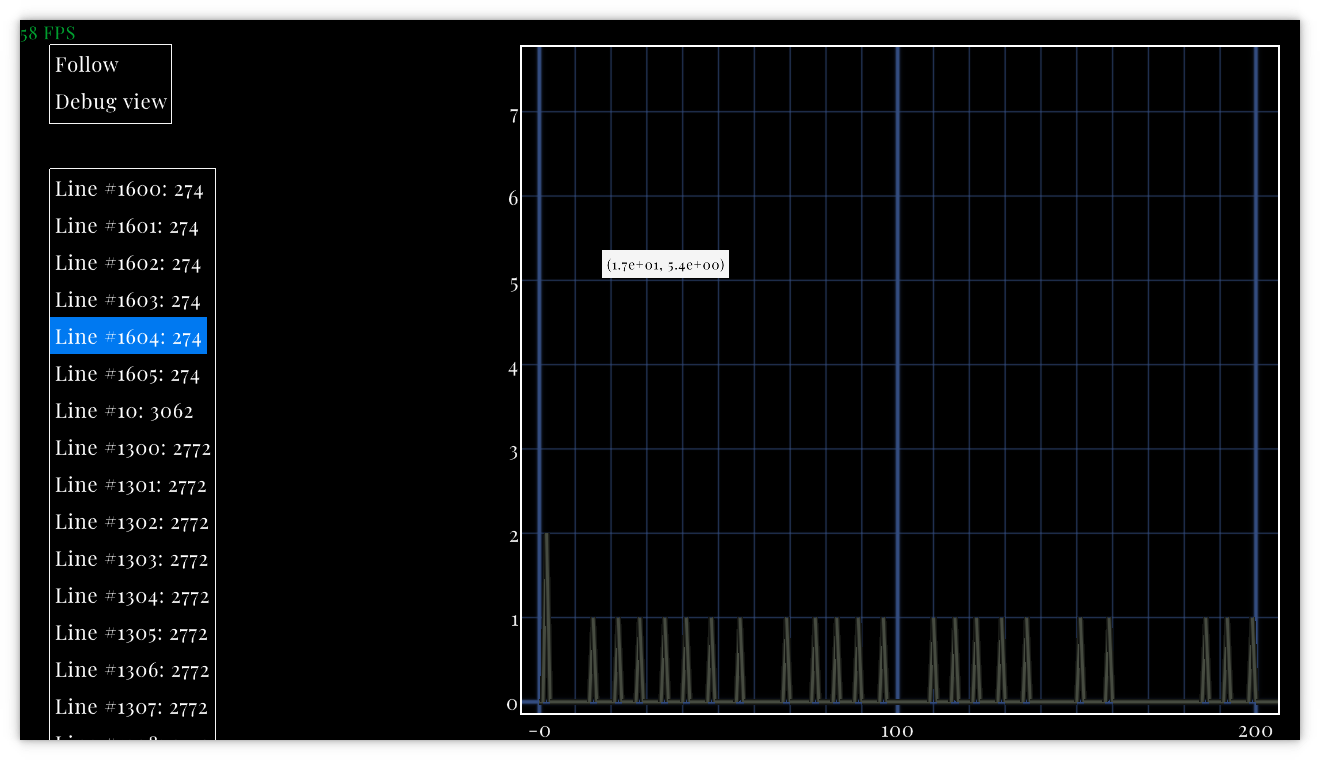
\includegraphics[width=2.8in]{q_full_ro_every_6ms.png}} &
    \subfloat[5ms]{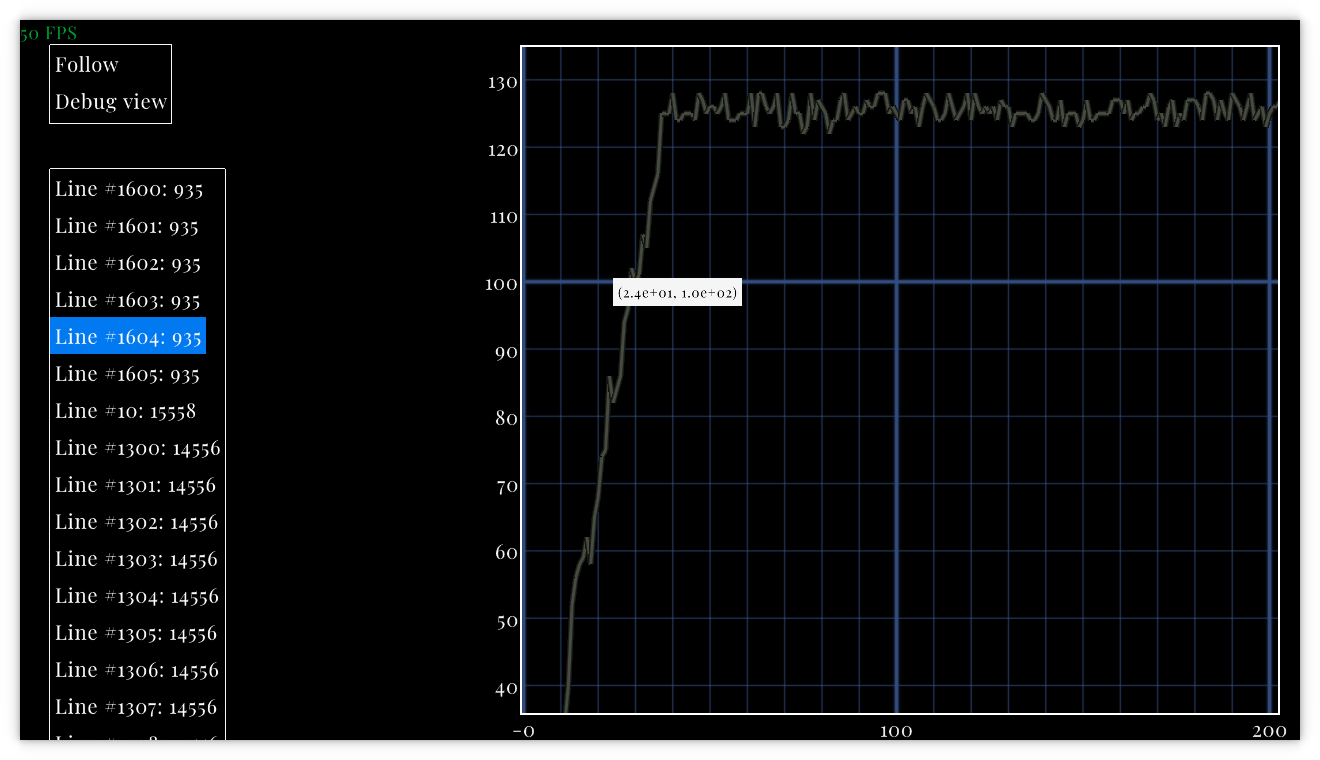
\includegraphics[width=2.8in]{q_full_ro_every_5ms.png}} \\
  \end{tabular}
  \caption{Broj elementa u strukturi koja ima oblik reda uzevši u obzir interval očitavanja podataka}
  \label{fig:q_full}
\end{figure}
Može se primjetiti da broj elementa ostaje minimalan sve dok interval očitavanja nije kraći od 6 milisekundi.

Provedena su dva dodatna mjeranja s intervalom očitanja od 5ms, jedno mjerenje s intervalom očitanja od 4ms i jedno mjerenje s itervalom očitanja 6ms uz udaljavanje i približavanj mikroupravljača od računala dok se provodilo mjerenje.
Slika \ref{fig:q_full_1} prikazuje ta mjerenja.

\begin{figure}[H]
  \begin{tabular}{cc}
    \subfloat[5ms]{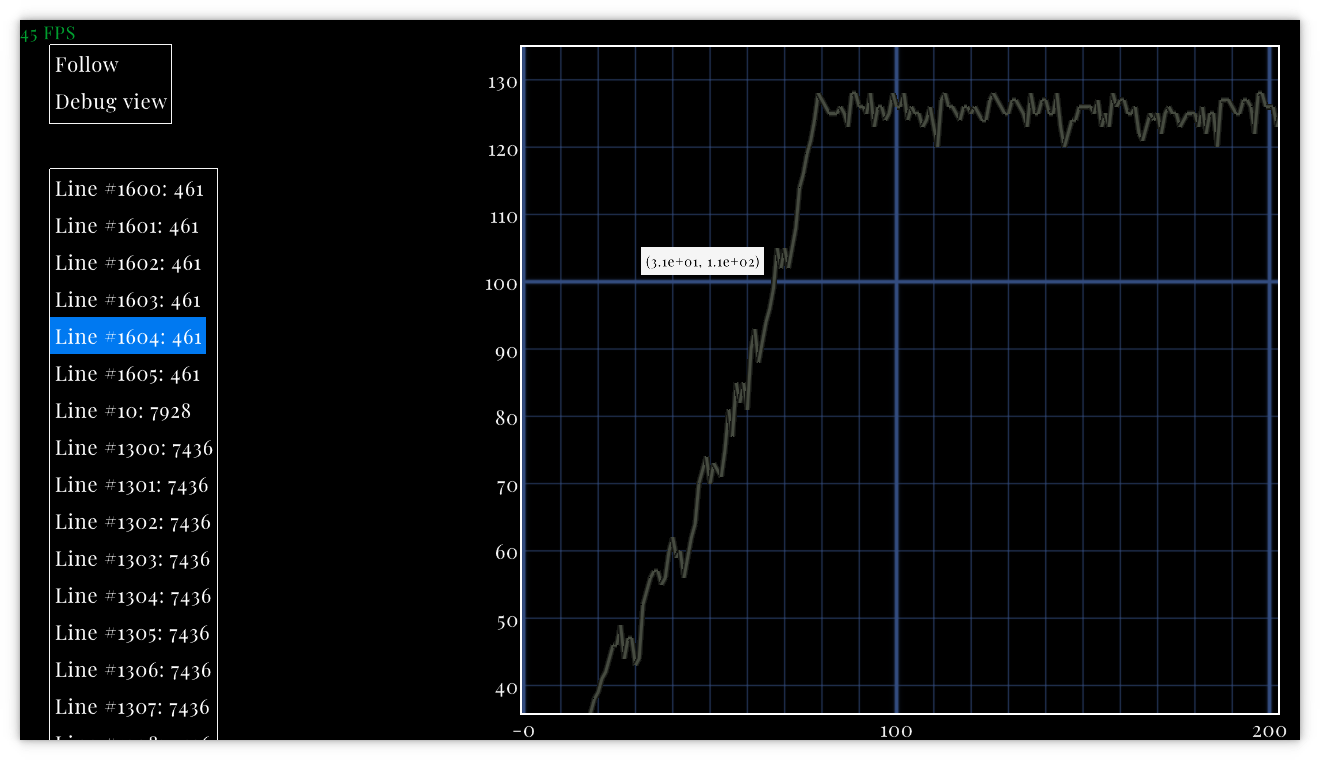
\includegraphics[width=2.8in]{q_full_ro_every_5ms_v2.png}} &
    \subfloat[5ms]{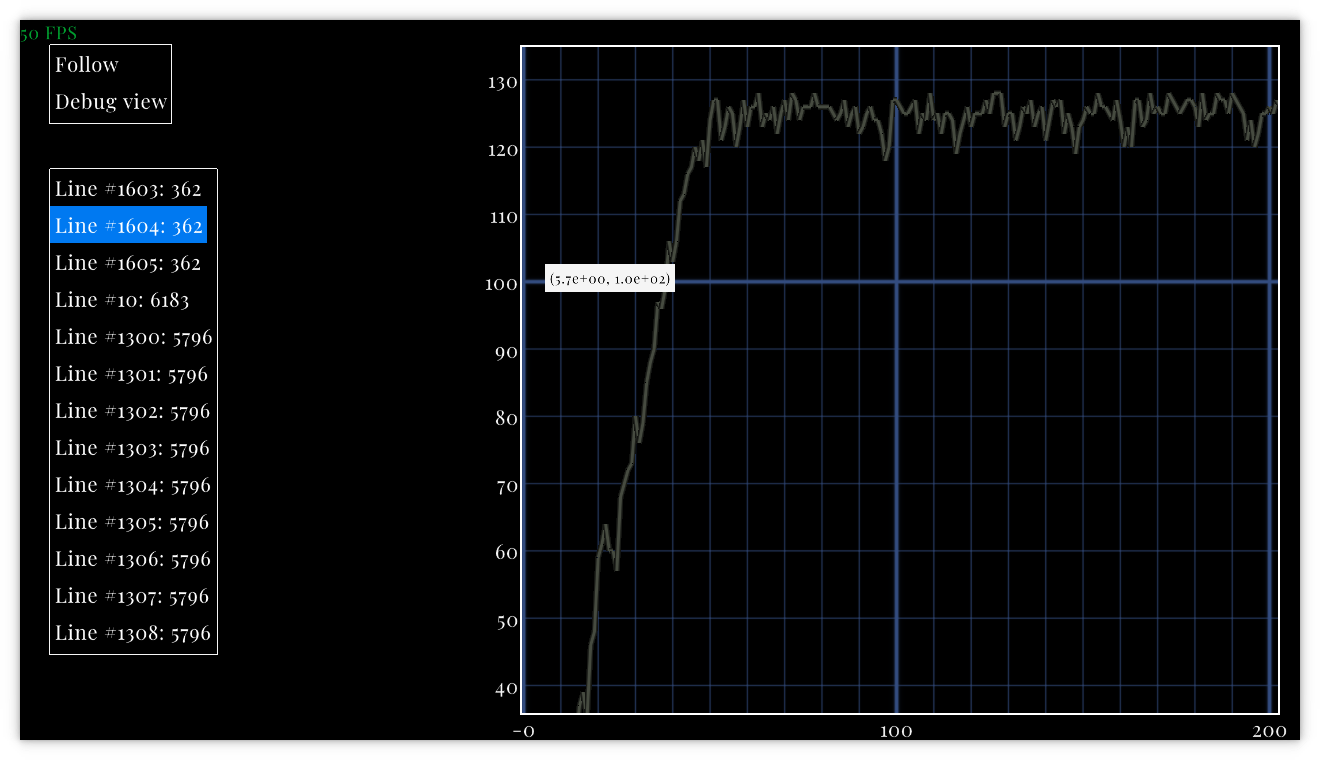
\includegraphics[width=2.8in]{q_full_ro_every_5ms_v3.png}} \\
    \subfloat[4ms]{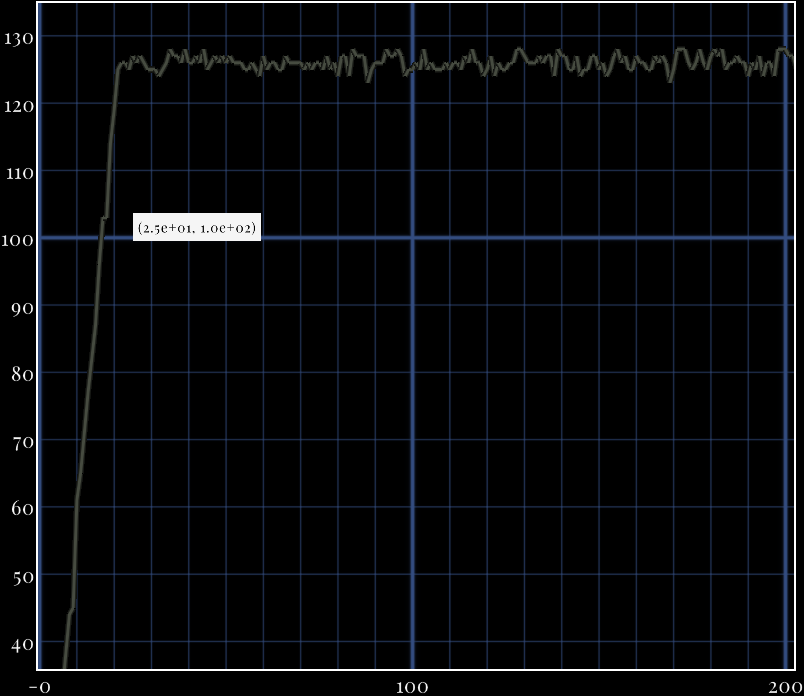
\includegraphics[width=2.8in]{q_full_ro_every_4ms.png}} &
    \subfloat[6ms uz udaljavanje]{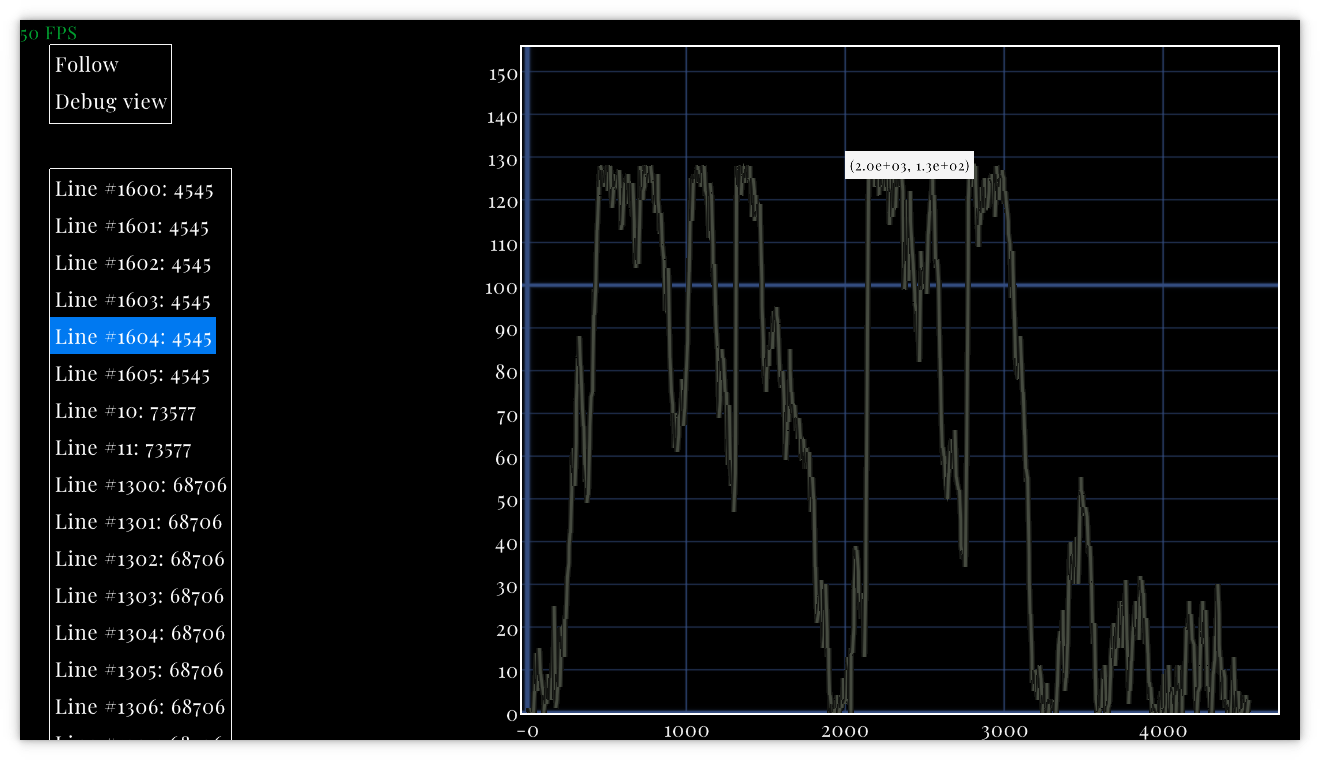
\includegraphics[width=2.8in]{q_full_ro_every_6ms_with_walking.png}}
  \end{tabular}
  \caption{Broj izgubljenih paketa uz brzinu očitanja podataka od 5ms i 6ms}
  \label{fig:q_full_1}
\end{figure}

Na slici \ref{fig:q_full_1} se može primjetiti da uz interval očitavanja od 5ms i 4ms broj elemenata raste do kapaciteta strukture koja ima oblik reda i nakon toga nastavlja biti u blizini te vrijednosti.
Dodatno, može se primjetiti da uz interval očitavanja od 6ms uz udaljavanje broj elemenata raste u trenucima kad je mikroupravljač udanjen od računala, ali nakon što se ponovno približi, broj elemenata počne padati.

\chapter{Razvojno okruženje}
U ovom radu korišteno je slobodno i otvoreno razvojno okruženje (engl. \textit{FLOSS} \cite{FLOSS}). Integrirana okruženja poput STM32CUBE omogućuju brz razvoj programskog rješenja. Cijena brzog razvoja nije direktno novčana, često takva integrirana razvojna rješenja imaju cijenu od 0€. Valuta plaćanju kod korištenja takvih sustava je sloboda. Sloboda mijenjanja tvrtke čiji se mikrokontroleri koriste. Jednom kad se programsko rješenje razvije u jednom od ne slobodnih integriranih okruženja, teško je to isto rješenje preformulirati da radi na uređajima koje proizvodi druga tvrtka \cite{VENDORLOCKIN}. Dodatna cijena koja se plaća korištenjem, specifično STM32CUBE integriranog okruženjem, je generiran kod koji nije zadovoljavajući. Naime, STM32CUBE često generira kod koji je previše općenit i rezultira većom potrošnjom memorije, sporijim izvođenjem i lošijom čitljivošću. Primjer takvog koda prikazan je u \ref{badcode}.

\lstinputlisting[caption={Primjer generiranog koda kojeg generira STM32CUBE IDE}, label={badcode}, basicstyle={\ttfamily\footnotesize\tiny}]{shitcode.c}

Svrha navedenog generiranog isječka koda je čitanje jednog okteta koji označava ime SPI poduređaja. Postoji pet indirekcija između pozivatelja funkcije i krajnje funkcije koja izvršava logiku čitanja tog okteta. Također, prilikom svakog poziva zadnje funkcije provjerava se koristi li se SPI ili I\(^2\)C. Provjera koji protokol se koristi izvršava se i kod svakog drugog poziva prema SPI poduređaju. Dodatno, niti jedan poduređaj nije moguće spojiti ni na koji drugi način osim korištenjem SPI protokola.

\subsubsection{cmake}
Cmake je programski alat koji je koristan za definiranje koraka potrebnih za izradnju projekta. U ovom radu koristi se za izradnju ugradbenog programa (engl. \textit{firmware}.) Cmake olakšava definiranje ovisnosti između jedinica prevođenja (engl. \textit{compilation units}.) Definiranje koje jedinice je potrebno prevesti ako se promjeni \textbf{header} datoteka. Dodatno osigurava konzistentnost postavljanja zastavica (engl. \textit{compilation flags}) u različitim jedinicama prevođenja.

\subsubsection{make}
GNU make je programski alat za definiranje \textit{recepta} i kako izraditi pojedini element sustava. U ovom projektu koristi se za automatizaciju, ne više od, pet \textbf{shell} naredbi koje se moraju izvršiti za gradnju neke komponente sustava. Primjer make recepta koji gradi ovu dokumentaciju pokretanjem \LaTeX \cite{ungar2002uvod} naredbi prikazan je u kodu \ref{lst:make}. Recept se čita ovako: \textit{Za izradnju pdf-a potreban je tex file. Ako je tex datoteka novija od pdf datoteke pokreni naredbe koje su ispod.} GNU make je besplatan alat s otvorenim izvornim kodom.

\begin{lstlisting}[language=make, label={lst:make}, caption={Gradnja dokumentacije korištenjem make recepta}]
build/docs/diplomski.pdf: docs/diplomski.tex
	cd docs && cp -R * ../build/docs && cd ../build/docs && pdflatex -mltex diplomski.tex && bibtex diplomski && pdflatex -mltex diplomski.tex
\end{lstlisting}

\subsubsection{OpenOCD}
OpenOCD \cite{openocd} je program koji se koristi za prebacivanje izvršne datoteke na mikrokontroler. Uz to omogućuje stvaranje GDB servera na koji moguće povezati s običnim GDB klijentima. OpenOCD je besplatan alat s otvorenim izvornim kodom.

\subsubsection{GDB}
GNU GDB \cite{gdb} je program koji pomaže programeru otkriti greške u kodu. GDB je besplatan alat s otvorenim izvornim kodom.

\subsubsection{GCC Arm}
GCC Arm \cite{armgcc} je alat koji pomaže programeru pretvoriti izvorni kod pisan u C programskom jeziku u binarni format kojeg je u konačnici moguće pokrenuti na mikrokontrolerima s ARM procesorom. Ustvari ovo je samo druga verzija(engl. \textit{fork}) GCC \cite{gcc} programa, verzija koja je specijalizirana za ARM procesore.

\subsubsection{Upute za pokretanje}
Za izranju i pokretanje sustava opisanog u ovom radu potrebo je slijediti sljedeće uputu:

\begin{itemize}
  \item Preuzeti izvorni kod sa stranice \url{https://github.com/branc116/diplomski}
  \item Pokrenuti gradnju izvršne datoteke naredbom \textit{make}
  \item Slanje izvršne datoteke na STM32L4 mikroupravljač
\end{itemize}

\chapter{Zaključak}
Stvaranje pouzdanog sustava zahtijeva poznavanje svake komponente sustava.
Bez poznavanja svake komponente nemoguće je donijeti zaključak radi li sustav ispravno.
Upoznavanje sa svakim dijelom sustava iziskuje najviše vremena.
Korištenje gotovih rješenja može ubrzati proces gradnje, ali bez razumijevanja svih komponenti gotovih rješenja teško se može razmatrati pouzdanost.
S druge strane stvaranje proizvoda iziskuje puno vremena, dubinsko upoznavanje svih komponenta dodatno usporava proces gradnje.
Potrebno je ponekad pouzdati se u gotove dijelove sustava i zanemariti pouzdanost.
Zbog svega navedenog, stvaranje pouzdanih sustava nije nimalo jednostavno, ali proces gradnje je zanimljiv i uvijek postoji nova stvar koja se može izučiti.

\nocite{*}
\bibliographystyle{diplomski}
\bibliography{diplomski}

\listoffigures

\lstlistoflistings


\begin{sazetak}
Ugradbena računala nude brojne mogućnosti poboljšanja svakodnevice pojedinaca. Njihove fizičke dimenzije i niska potrošnja čine ih dobrim kandidatom za stvaranjem uređaja i strojeva koji su pametniji od onih proizvedenih u prošlom desetljeću. Iako je bolja budućnost veoma blizu svima nama i iako postoje ugradbena računala koja nam omogućuju izradnju pametnijih stvari, proces izradnje nije nimalo trivijalan. Ovaj se rad bavi navedenim procesom i analizom pouzdanosti istog.

\kljucnerijeci{Ugradbena računala, Pouzdanost, Bluetooth, STM32}
\end{sazetak}

\engtitle{Software support for data collection from embedded devices with high availability}

\begin{abstract}
Embedded computers offer number of features that can augment day to day existence of every individual. Their dimensions and power efficiency make them great candidate for making a world a better place. Even thou embedded devices exist and are available to everyone, creating a system that uses that device is not trivial. This work touches on those processes and analysis of availability of those processes.

\keywords{Embedded Computers, Availability, Bluetooth, STM32}
\end{abstract}

\end{document}
